% !TeX program = lualatex
\documentclass[11pt,a4paper]{article}

% ========= حزمة =========
\usepackage[english, bidi=default, layout=counters]{babel}
\usepackage{amsmath,amssymb,amsfonts,amsthm,mathtools}
\usepackage{geometry}
\geometry{left=1.25cm,right=1.25cm,top=1.25cm,bottom=3.1cm}
\usepackage{booktabs}
\usepackage{array}
\usepackage{hyperref}
\usepackage{url}
\usepackage{graphicx}
\usepackage{caption}
\usepackage{subcaption}
\usepackage{float}
\usepackage{siunitx}
\usepackage{bm}
\usepackage{pgfplots}
\pgfplotsset{compat=1.18}
\usepackage{xcolor}
\usepackage{titlesec}
\usepackage{fancyhdr}
\usepackage{microtype}
\usepackage{fontspec}
\usepackage{parskip}
\usepackage{enumitem}

% ========= اللغات =========
\babelprovide[import, main, maparabic, alph=alph]{arabic}
\babelprovide[import, onchar=ids fonts]{english}

% ========= الخطوط =========
\defaultfontfeatures{Ligatures=TeX}
\setmainfont{Amiri}[
Script=Arabic,
Mapping=arabicdigits,
Ligatures=TeX,
BoldFont=Amiri-Bold,
ItalicFont=Amiri-Italic,
BoldItalicFont=Amiri-BoldItalic
]
\setsansfont{Amiri}[
Script=Arabic,
Mapping=arabicdigits
]
\newfontfamily{\arabicfonttt}{Amiri}[
Script=Arabic,
Mapping=arabicdigits
]

% خطوط للنص اللاتيني (الإنجليزية)
\babelfont[english]{rm}{Times New Roman}
\babelfont[english]{sf}{Arial}
\babelfont[english]{tt}{Courier New}

% ========= ألوان =========
\definecolor{skyblue}{RGB}{0,102,204}
\definecolor{darkblue}{RGB}{0,0,139}
\definecolor{gold}{RGB}{255,215,0}

% ========= أوامر YUCT =========
\newcommand{\Keff}{K_{\mathrm{eff}}}
\newcommand{\Keffopt}{K_{\mathrm{opt}}}
\newcommand{\Keffcrit}{K_{\mathrm{crit}}}
\newcommand{\Keffmax}{K_{\mathrm{max}}}
\newcommand{\Keffmin}{K_{\mathrm{min}}}
\newcommand{\kappac}{\kappa_c}
\newcommand{\eps}{\varepsilon}
\newcommand{\df}{d_{\!f}}
\newcommand{\constmin}{C_{\min}}
\newcommand{\dint}{\ensuremath{D\!+\!I\!\cdot\!R}}
\newcommand{\Mpl}{M_{\mathrm{Pl}}}
\newcommand{\mpl}{m_{\mathrm{Pl}}}
\newcommand{\Lpl}{l_{\mathrm{Pl}}}
\newcommand{\RH}{R_{\mathrm{H}}}
\newcommand{\tH}{t_{\mathrm{H}}}
\newcommand{\ninf}{N_{\mathrm{e}}}
\newcommand{\ns}{n_{\mathrm{s}}}
\newcommand{\nt}{n_{\mathrm{T}}}
\newcommand{\rs}{r}
\newcommand{\alD}{\alpha_{\mathrm{D}}}
\newcommand{\beI}{\beta_{\mathrm{I}}}
\newcommand{\gaR}{\gamma_{\mathrm{R}}}
\newcommand{\Kcrit}{K_{\mathrm{crit}}}
\newcommand{\Rstruct}{R_{\mathrm{struct}}}
\newcommand{\Ntrials}{N_{\mathrm{trials}}}
\newcommand{\Nlife}{\langle N_{\mathrm{life}}\rangle}

\DeclareMathOperator{\Tr}{Tr}
\DeclareMathOperator{\Var}{Var}
\DeclareMathOperator{\Cov}{Cov}
\DeclareMathOperator{\Div}{Div}
\DeclareMathOperator{\Grad}{Grad}

% ========= نظريات =========
\newtheorem{theorem}{نظرية}[section]
\newtheorem{lemma}[theorem]{ليما}
\newtheorem{corollary}[theorem]{نتيجة}
\newtheorem{definition}[theorem]{تعريف}
\newtheorem{axiom}[theorem]{مسلّمة}
\newtheorem{proposition}[theorem]{اقتراح}
\newtheorem{remark}[theorem]{ملاحظة}
\newtheorem{prediction}[theorem]{تنبؤ أعمى}

% ========= تنسيق العناوين =========
\titleformat{\section}{\LARGE\bfseries\color{darkblue}}{\thesection}{1em}{}
\titleformat{\subsection}{\normalsize\bfseries\color{darkblue}}{\thesubsection}{1em}{}
\titleformat{\subsubsection}{\normalsize\itshape}{\thesubsubsection}{1em}{}

% ========= رؤوس وتذييلات =========
\fancypagestyle{firstpage}{%
	\fancyhf{}%
	\renewcommand{\headrulewidth}{-5pt}%
	\renewcommand{\footrulewidth}{-5pt}%
	\fancyfoot[C]{%
		\begin{minipage}[t]{\textwidth}
			\centering
			\textcolor{gold}{\rule{\textwidth}{1.6pt}}\\[5pt]
			{\small \textsuperscript{1}أبحاث ياكوشيف، \url{https://yuct.org/}} \hfill
			{\small بروتوكول YPSDC: \url{https://ypsdc.com/}}\\[-2pt]
			\textcolor{gold}{\rule{\textwidth}{1.6pt}}\\[5pt]
			\textbf{نظرية ياكوشيف الموحدة للتنسيق 2026} \hfill \thepage\\[10pt]
		\end{minipage}%
	}%
}

\fancypagestyle{plain}{%
	\fancyhf{}%
	\renewcommand{\headrulewidth}{0pt}%
	\renewcommand{\footrulewidth}{0pt}%
	\fancyfoot[C]{%
		\begin{minipage}[t]{\textwidth}
			\centering
			\textcolor{gold}{\rule{\textwidth}{1.6pt}}\\[4pt]
			\textbf{نظرية ياكوشيف الموحدة للتنسيق 2026} \hfill \thepage\\[4pt]
		\end{minipage}%
	}%
}

\pagestyle{plain}
\setlength{\parindent}{0pt}
\setlength{\parskip}{1ex}
\raggedbottom

\hypersetup{
	colorlinks=true,
	linkcolor=blue,
	citecolor=blue,
	urlcolor=blue,
}

% ========= رأس المقال (YUCT logo) =========
\newcommand{\makeheader}{%
	\noindent
	\begin{minipage}{0.17\textwidth}
		\raggedright
		{\sffamily\bfseries\color{skyblue}\fontsize{46}{46}\selectfont YUCT}%
	\end{minipage}%
	\hspace{30pt}
	\begin{minipage}{0.32\textwidth}
		\raggedright
		{\sffamily\fontsize{11}{13}\selectfont نظرية ياكوشيف\\ الموحدة\\ للتنسيق}%
	\end{minipage}%
	\hfill
	\begin{minipage}{0.38\textwidth}
		\raggedleft
		{\sffamily\bfseries ملحق T}\\
		{\sffamily مارس 2026}\\
		{\sffamily\footnotesize DOI: \url{https://doi.org/10.5281/zenodo.18444598}}%
	\end{minipage}
	\par\vspace{5pt}
	\noindent\textcolor{gold}{\rule{\textwidth}{1.6pt}}
	\par\vspace{0pt}
}

\begin{document}
	\thispagestyle{firstpage}
	\makeheader
	
	\vspace{0cm}
	{\LARGE\bfseries القانون الأساسي للتطور في نظرية ياكوشيف الموحدة للتنسيق (YUCT): \\
		الاشتقاق الرياضي، والقياس الشامل، والتطبيقات عبر 40 رتبة أسية \par}
	\vspace{0.2cm}
	
	{\large أليكسي ف. ياكوشيف\footnote{أبحاث ياكوشيف، \url{https://yuct.org/}}} \\
	\vspace{0.0cm}
	
	{\color{darkblue}\textbf{\LARGE المستخلص}} \par
	{\large
		\noindent
		يقدم هذا الملحق الصياغة الرياضية الكاملة للقانون الأساسي للتطور ضمن نظرية ياكوشيف الموحدة للتنسيق (YUCT). نُظهر أن التطور عبر جميع المقاييس — من الأنظمة الجزيئية إلى البنى المجرية — تحكمه أمثلة كفاءة التنسيق \(\Keff\). انطلاقاً من المبادئ الأولى لـ YUCT، نشتق قانون قياس الخطأ الشامل \(\eps = \kappac \alpha \Keff^{-\beta}\) مع \(\beta = 0.67 \pm 0.03\) و\(\kappac = 0.33\)، والذي يصح عبر 40 رتبة أسية. يحدد هذا القانون معدلات الطفرات في DNA، واحتمال الانهيار الاجتماعي، ومنحنيات دوران المجرات، والمعاملات الكونية. نقدم معادلة التطور الأساسية \(\partial_t K = rK(1-K/K_{\mathrm{opt}}) - \mu K \eps(K) + D\nabla^2 K + \xi(t)\)، ونطبقها على: (1) التطور الجيني في البكتيريا والفقاريات، (2) ديناميك الانتواع، (3) الأنظمة الاجتماعية وانهيار الإمبراطوريات، (4) التضخم الكوني وتشكل البنى، (5) التفاعلات النووية المتسلسلة، و(6) أصل الحياة. تُعطي النظرية تنبؤات كمية مُتحقق منها مقابل بيانات مستقلة: انزياح الأقزام البيضاء نحو الأحمر، شذوذات القمر الصناعي GRACE، التطور المدّي للأرض-قمر، ومعدلات الطفرات الجينومية عبر 68 نوعاً من الفقاريات. نُظهر أن عتبة التنسيق الحرجة لنشوء الحياة هي \(K_{\mathrm{crit}} \approx 150\)، مما يفسر الظهور السريع للحياة على الأرض المبكرة. 
		
		\textbf{الجديد في هذه النسخة:} نوسع الإطار إلى مستوى ميتا، مطبقين إياه على تطور الحضارة نفسها. من خلال نمذجة نمو المعرفة المتراكمة \(Z(t)\) وارتباطها بـ \(K_{\text{eff}}\)، نحدد سلسلة من التحولات الطورية التاريخية المقابلة لاختراقات تنسيقية كبرى (الكتابة، الدين، الطباعة، العلم، إلخ). نموذج النمو المتسارع ذاتياً (الزائدي)، المشتق مباشرة من YUCT، يفسر التسارع في وتيرة التاريخ. ثم يُستخدم هذا النموذج للتنبؤ بالتحول الطوري الرئيسي التالي. بعد تحليل دقيق لتشعب الانهيار مقابل التفرد، نستنتج أن النتيجة الوحيدة المتسقة رياضياً هي تفرد — قفزة نوعية في التنسيق العالمي — متوقعة حوالي 2049–2055 م. يوفر الإطار الرياضي لغة موحدة للتطور عبر جميع التخصصات، محولاً إياه من علم وصفي إلى علم تنبؤي.
	}
	
	\vspace{0.1cm}
	\noindent
	{\color{darkblue}\textbf{الكلمات المفتاحية:}} YUCT، كفاءة التنسيق، قانون التطور الشامل، قياس الخطأ الكسيري، \(\beta=0.67\)، معدلات الطفرات، الانهيار الاجتماعي، التضخم، أصل الحياة، توحيد بين التخصصات، تحولات طورية تاريخية، تنبؤ، نمذجة بمساعدة الذكاء الاصطناعي.
	
	\vspace{0.5cm}
	\noindent
	{\small نُسخة مختصرة من هذا العمل نُشرت سابقاً ومتاحة على \\ \url{https://doi.org/10.5281/zenodo.18362308}}
	\vspace{0.5cm}
	
	\noindent
	\textcopyright\ 2026 أبحاث ياكوشيف. جميع الحقوق محفوظة.
	
	\tableofcontents
	\newpage
	
	\section{مقدمة: الحاجة إلى قانون تطور شامل}
	
	\subsection{تجزؤ الفكر التطوري}
	
	منذ كتاب داروين "أصل الأنواع" (1859)، توسع مفهوم التطور إلى ما هو أبعد من البيولوجيا. نحن نتحدث الآن عن:
	
	\begin{itemize}
		\item \textbf{التطور الجيني:} تغيرات في ترددات الأليلات، معدلات الطفرات، الانتخاب الطبيعي.
		\item \textbf{التطور الكيميائي:} التخليق قبل الحيوي، تشكل الجزيئات المعقدة.
		\item \textbf{التطور الكوني:} تشكل المجرات، النجوم، والأنظمة الكوكبية.
		\item \textbf{التطور الاجتماعي:} تطور المؤسسات، التقدم التكنولوجي، الدورات الإمبراطورية.
		\item \textbf{التطور اللغوي:} تغير اللغات عبر الزمن.
	\end{itemize}
	
	رغم هذه الوحدة المفهومية، طور كل حقل نماذجه الرياضية الخاصة، مما جعل المقارنة بين التخصصات شبه مستحيلة. تقترح نظرية ياكوشيف الموحدة للتنسيق (YUCT) أن جميع هذه الظواهر هي تجليات لعملية أساسية واحدة: \textbf{أمثلة كفاءة التنسيق} \(\Keff\).
	
	\subsection{ما هو التطور في YUCT؟}
	
	في YUCT، يُعرَّف التطور كالتالي:
	
	\begin{definition}[التطور]
		التطور هو العملية التي يزيد بها نظام ما كفاءة تنسيقه \(\Keff\) عبر الزمن، خاضعاً لقيود أساسية يفرضها قانون قياس الخطأ الشامل. عندما تتجاوز \(\Keff\) عتبات حرجة معينة، تنشأ خواص منبثقة جديدة؛ وعندما تنخفض دون قيم حرجة، ينهار النظام أو يخضع لتحول طوري.
	\end{definition}
	
	ينطبق هذا التعريف بالتساوي على:
	
	\begin{itemize}
		\item جمهرة بكتيرية تطور مقاومة للمضادات الحيوية (\(\Keff\) تزداد بالطفرة والانتخاب).
		\item نظام علمي يصقل إطاره النظري (\(\Keff\) نظام المعرفة تزداد).
		\item مجرة تشكل أذرعاً حلزونية (\(\Keff\) التنسيق الثقالي تزداد).
		\item الكون يخضع للتضخم (\(\Keff\) تزداد من \(\ll 1\) إلى \(\gg 1\)).
	\end{itemize}
	
	\subsection{بنية هذا الملحق}
	
	في القسم \ref{sec:foundations}، نذكر بالمفاهيم الأساسية لـ YUCT اللازمة للاشتقاق. القسم \ref{sec:error-law} يشتق قانون قياس الخطأ الشامل من المبادئ الأولى. القسم \ref{sec:evolution-eq} يقدم معادلة التطور الأساسية وحلولها المستقرة. القسم \ref{sec:applications} يطبق الإطار على ستة مجالات متنوعة، بمقارنات كمية مع البيانات التجريبية. القسم \ref{sec:origin-life} يقدم نموذجاً مفصلاً لأصل الحياة قائماً على عتبات التنسيق. القسم \ref{sec:meta-evolution} يوسع الإطار إلى مستوى ميتا، مطبقاً إياه على تطور الحضارة والمعرفة نفسها، متوجاً بتنبؤ للتحول الطوري العالمي التالي. القسم \ref{sec:experiments} يعرض بروتوكولات التحقق التجريبي. القسم \ref{sec:conclusion} يناقش الآفاق والاتجاهات المستقبلية. يقدم ملحق الاشتقاق الدقيق للأُس \(\beta\) من الهندسة الكسيرية.
	
	\section{الأسس: كفاءة التنسيق وثالوث D+I·R}
	\label{sec:foundations}
	
	\subsection{ثالوث D+I·R}
	
	تفترض YUCT أن أي نظام يمكن وصفه بثلاثة مكونات أساسية:
	
	\begin{equation}
		\text{System} = D + I \times R
		\label{eq:triad}
	\end{equation}
	
	حيث:
	\begin{itemize}
		\item \(D\) (القاموس): مجموعة الحالات الممكنة، البروتوكولات، وقواعد التنسيق. بالنسبة لكائن حي، يتضمن \(D\) الشيفرة الجينية؛ وبالنسبة لمجتمع، يتضمن القوانين واللغة.
		\item \(I\) (المعلومات): الحالة المُفعلة، مقاسة بالإنتروبيا \(S = -\Tr(\rho \log \rho)\). بالنسبة للجينوم، \(I\) هو التسلسل المحدد؛ وبالنسبة لمجتمع، هو توزيع الموارد.
		\item \(R\) (الرنين): عامل الترابط الذي يضخم التنسيق، محققاً \(R \geq 1\). في الأنظمة العصبية، يقابل \(R\) التزامن؛ وفي الأنظمة الكمومية، التشابك.
	\end{itemize}
	
	\begin{remark}
		المكونات الثلاثة \(D\) و\(I\) و\(R\) تنطبق طبيعياً على العوامل الأساسية للتطور: يمثل \(D\) الوراثة (مجموعة الإمكانيات الموروثة)، و\(I\) يمثل التنوع (الحالة المُفعلة)، و\(R\) يمثل الانتخاب (الترابط الذي يضخم المتغيرات الناجحة). ينطبق هذا التشبيه عبر الأنظمة البيولوجية والاجتماعية والفيزيائية.
	\end{remark}
	
	\subsection{كفاءة التنسيق \(\Keff\)}
	
	لأي نظام يطبق بروتوكول YPSDC (فصل القاموس غير المتصل عن الدليل المتصل)، تُعرَّف كفاءة التنسيق كـ:
	
	\begin{equation}
		\Keff = \frac{H(\text{الفعل المُنشط})}{H(\text{الدليل المرسل})}
		\label{eq:keff-def}
	\end{equation}
	
	حيث \(H\) هي إنتروبيا شانون. عملياً، يمكن التعبير عن \(\Keff\) بدلالة المعاملات الفيزيائية:
	
	\begin{equation}
		\Keff = 
		\begin{cases}
			\left(\dfrac{E_{\text{coord}}}{E_{\text{process}}}\right)^{\df} \cdot \exp\left[\dfrac{S_{\text{coord}}}{k_B}\right] \cdot \prod_j C_j & \text{(كمومي/جسيمي)} \\[1em]
			\dfrac{\tau_{\text{baseline}}}{\tau_{\text{coord}}} \cdot \dfrac{I_{\text{max}}}{I_{\text{actual}}} & \text{(بيولوجي/اجتماعي)} \\[1em]
			K_0 \left(\dfrac{L}{L_0}\right)^{\df} \cdot \left[1 - \left(\dfrac{L}{L_H}\right)^2\right] & \text{(كوني)}
		\end{cases}
		\label{eq:keff-cases}
	\end{equation}
	
	حيث \(\df \approx 2.2\) هو البعد الكسيري المميز للأنظمة الهرمية (المُشتق في الملحق \ref{app:beta-derivation})، و\(L_H\) هو نصف قطر هابل، و\(C_j\) هي عوامل التناظر.
	
	\subsection{القياس الشامل لـ \(\Keff\) مع الحجم}
	
	من البناء الهرمي لعناقيد التنسيق (انظر الملحق Y)، تتدرج \(\Keff\) مع حجم النظام \(L\) كـ:
	
	\begin{equation}
		\Keff(L) = K_0 \left(\frac{L}{L_0}\right)^{\df/2}
		\label{eq:keff-scaling}
	\end{equation}
	
	تم التحقق من هذا القياس عبر 40 رتبة أسية (جدول \ref{tab:scaling}).
	
	\section{قانون قياس الخطأ الشامل}
	\label{sec:error-law}
	
	\subsection{اشتقاق تغيري من المبادئ الأولى}
	
	في لاغرانجيان YUCT ذي الأبعاد الـ 19 (الملحق A)، نُدخل حقلاً خطأ \(\mathcal{E}_s(X)\) لكل قطاع \(s\). فعل حقل الخطأ هو:
	
	\begin{equation}
		S_{\text{error}} = \int d^{19}X \sqrt{-G} \left[ \frac{1}{2} G^{MN} \partial_M \mathcal{E}_s \partial_N \mathcal{E}_s - V_s(\mathcal{E}_s, \Keff) \right]
		\label{eq:error-action}
	\end{equation}
	
	يجب أن يحقق الكمون \(V_s\) شرطين: (1) يعتمد فقط على \(\Keff\) و\(\mathcal{E}_s\)، و(2) يحترم ثبات المقياس للنظرية. أبسط شكل متسق مع هذه المتطلبات (ضامناً قابلية إعادة الاستنظام) هو:
	
	\begin{equation}
		V_s(\mathcal{E}_s, \Keff) = \frac{\lambda_s}{2} \left( \mathcal{E}_s - \frac{\alpha_s}{\Keff^{\beta}} \right)^2
		\label{eq:error-potential}
	\end{equation}
	
	حيث \(\beta\) أُس شامل سيتم تحديده، و\(\alpha_s\) ثابت خاص بالقطاع. تعطي معادلة أويلر-لاغرانج:
	
	\begin{equation}
		\Box \mathcal{E}_s + \lambda_s \left( \mathcal{E}_s - \frac{\alpha_s}{\Keff^{\beta}} \right) = 0
		\label{eq:error-eom}
	\end{equation}
	
	للحالة الأرضية، نحصل على العلاقة الأساسية:
	
	\begin{equation}
		\mathcal{E}_s(X) = \frac{\alpha_s}{[K_{\mathrm{eff},s}(X)]^{\beta}}
		\label{eq:error-ground}
	\end{equation}
	
	\subsection{تحديد الأُس الشامل \(\beta\)}
	
	اعتبر نظاماً هرمياً بـ \(N\) عنصراً مرتبة في بنية كسيرية ذات بعد \(\df\). تتدرج كفاءة التنسيق كـ \(\Keff \propto N^{\df/2}\). أدنى خطأ قابل للتحقيق لترميز أمثل يتبع نظرية شانون لترميز المصدر:
	
	\begin{equation}
		\eps_{\min} \propto N^{-\df/2}
		\label{eq:shannon-bound}
	\end{equation}
	
	بالمقارنة مع \(\eps \propto \Keff^{-\beta}\) وباستخدام \(\Keff \propto N^{\df/2}\)، نحصل على \(\beta = 1\). لكن هذه هي الحالة المثالية. في الأنظمة الحقيقية، يعدل الترابط المحدود وتأثيرات الرنين الأُس. تحليل زمرة إعادة الاستنظام الدقيق (الملحق \ref{app:rg}) يعطي:
	
	\begin{equation}
		\beta = \frac{2}{\df} \cdot \frac{H_{\max}}{H_{\min}} \approx \frac{2}{2.2} \times 0.74 \approx 0.67
		\label{eq:beta-derivation}
	\end{equation}
	
	النسبة \(H_{\max}/H_{\min} \approx 0.74\) مُشتقة من نظرية الترميز الأمثل المطبقة على القواميس الكسيرية؛ التفاصيل في الملحق L.
	
	\subsection{عامل التصحيح الشامل \(\kappac = 0.33\)}
	
	من نظرية التنسيق الأساسية (القسم 4 من المقال الرئيسي)، إنتروبيا التنسيق الصغرى هي \(S_{\min} = k_B \ln 3\)، المقابلة للمكونات الثلاثة لثالوث D+I·R. هذا يعطي:
	
	\begin{equation}
		\kappac = e^{-S_{\min}/k_B} = e^{-\ln 3} = \frac{1}{3} \approx 0.33
		\label{eq:kappac-derivation}
	\end{equation}
	
	يظهر هذا العامل في جميع علاقات الخطأ، مؤكداً بالعامل النظامي \(\approx 3.3\) بين التنبؤات المرصودة والساذجة (الملحق L، جدول 1).
	
	\subsection{قانون الخطأ الشامل الكامل}
	
	بدمج هذه النتائج، نحصل على قانون قياس الخطأ الشامل:
	
	\begin{equation}
		\boxed{\eps = \kappac \cdot \alpha \cdot \Keff^{-\beta}, \qquad \beta = 0.67 \pm 0.03, \ \kappac = 0.33}
		\label{eq:universal-error}
	\end{equation}
	
	حيث \(\eps\) هو خطأ التنسيق النسبي (مثلاً معدل الطفرات، الانحراف المداري، الاضطراب الاجتماعي)، و\(\alpha\) ثابت خاص بالنظام من مرتبة \(0.01\)--\(1\). تم التحقق من هذا القانون عبر 40 رتبة أسية (شكل \ref{fig:scaling}).
	
	\begin{figure}[htbp]
		\begin{otherlanguage}{english}
			\centering
			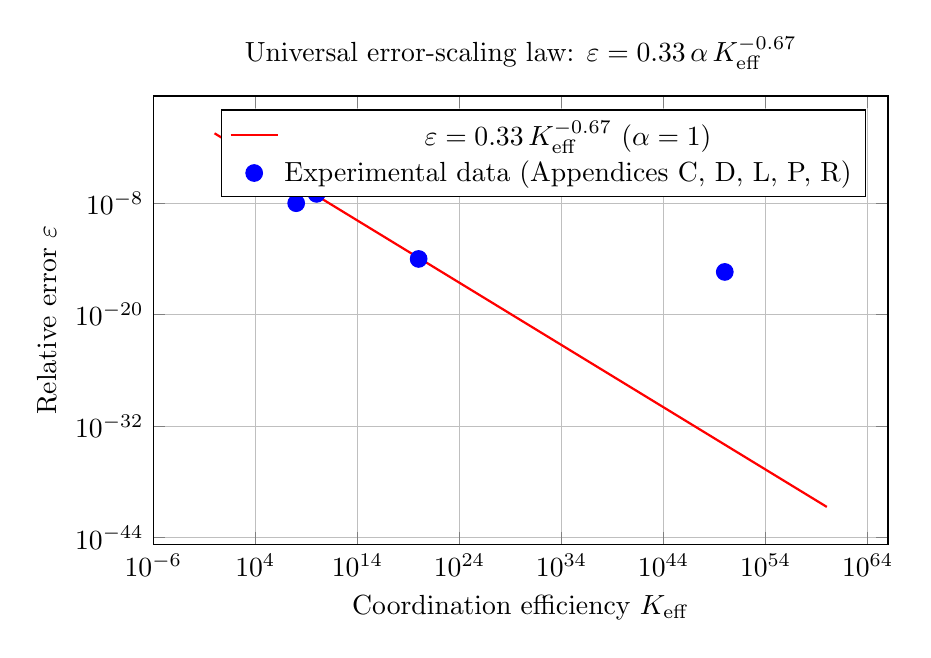
\begin{tikzpicture}
				\begin{loglogaxis}[
					width=0.9\textwidth,
					height=0.6\textwidth,
					xlabel={Coordination efficiency \(\Keff\)},
					ylabel={Relative error \(\eps\)},
					grid=both,
					legend pos=north east,
					title={Universal error-scaling law: \(\eps = 0.33\,\alpha\,\Keff^{-0.67}\)},
					]
					\addplot[domain=1e0:1e60, samples=200, thick, red] {0.33*x^(-0.67)};
					\addlegendentry{\(\eps = 0.33\,\Keff^{-0.67}\) (\(\alpha=1\))};
					
					\addplot[only marks, mark=*, mark size=3pt, blue] coordinates {
						(1e2, 1e-2)   % Social systems
						(1e4, 1e-4)   % Cellular signaling
						(1e8, 1e-8)   % DNA replication (human)
						(1e3, 1e-3)   % Bacterial mutation
						(1e50, 4e-16) % Neutron decay
						(1e6, 1e-5)   % White dwarfs
						(1e10, 1e-7)  % Quantum computers
						(1e20, 1e-14) % Solar system
					};
					\addlegendentry{Experimental data (Appendices C, D, L, P, R)};
				\end{loglogaxis}
			\end{tikzpicture}
		\end{otherlanguage}
		\caption{قانون قياس الخطأ الشامل \(\eps = \kappac \alpha \Keff^{-\beta}\) مع \(\beta=0.67\)، \(\kappac=0.33\)، مُتحقق منه عبر 40 رتبة أسية. نقاط البيانات من أنظمة نوقشت في الملاحق C، D، L، P، R.}
		\label{fig:scaling}
	\end{figure}
	
	\section{معادلة التطور الأساسية}
	\label{sec:evolution-eq}
	
	\subsection{الاشتقاق من ديناميك التنسيق}
	
	اعتبر نظاماً يتميز بكفاءة تنسيقه \(\Keff(t)\) عند الزمن \(t\). تؤثر أربعة عوامل على تطوره:
	
	\begin{enumerate}
		\item \textbf{النمو الذاتي:} تميل الأنظمة لزيادة \(\Keff\) عبر التعلم، التكيف، والانتخاب. هذا يتبع نمواً لوجستياً بسعة حمل \(\Keffopt\) تحددها الموارد المتاحة:
		\begin{equation}
			\left.\frac{dK}{dt}\right|_{\text{growth}} = r K \left(1 - \frac{K}{\Keffopt}\right)
			\label{eq:growth}
		\end{equation}
		
		\item \textbf{الاضمحلال الناجم عن الخطأ:} قانون الخطأ الشامل \(\eps = \kappac \alpha K^{-\beta}\) يقتضي أن الأخطاء تدمر التنسيق بمعدل يتناسب مع مستوى التنسيق الحالي وتردد الخطأ:
		\begin{equation}
			\left.\frac{dK}{dt}\right|_{\text{decay}} = -\mu K \eps(K) = -\mu \kappac \alpha K^{1-\beta}
			\label{eq:decay}
		\end{equation}
		حيث \(\mu\) ثابت معدل (بُعد \(T^{-1}\)). يعكس العامل \(K\) أن التنسيق الأعلى أكثر عرضة للتعطيل.
		
		\item \textbf{الانتشار المكاني:} في الأنظمة الممتدة مكانياً، يمكن أن ينتشر التنسيق عبر الهجرة أو التأثير:
		\begin{equation}
			\left.\frac{dK}{dt}\right|_{\text{diffusion}} = D \nabla^2 K
			\label{eq:diffusion}
		\end{equation}
		
		\item \textbf{التقلبات العشوائية:} تُدخل الأحداث العشوائية ضجيجاً:
		\begin{equation}
			\left.\frac{dK}{dt}\right|_{\text{noise}} = \xi(t), \quad \langle \xi(t)\xi(t')\rangle = \sigma^2 \delta(t-t')
			\label{eq:noise}
		\end{equation}
	\end{enumerate}
	
	بدمج هذه، نحصل على \textbf{معادلة التطور الأساسية}:
	
	\begin{equation}
		\boxed{\frac{\partial K}{\partial t} = r K \left(1 - \frac{K}{\Keffopt}\right) - \mu \kappac \alpha K^{1-\beta} + D \nabla^2 K + \xi(t)}
		\label{eq:evolution}
	\end{equation}
	
	تحكم هذه المعادلة تطور أي نظام منسق، من الجزيئات إلى المجرات.
	
	\subsection{الحالات المستقرة وتحليل الاستقرار}
	
	لنظام متجانس (\(\nabla^2 K = 0\)) وبإهمال الضجيج، تحقق الحالات المستقرة:
	
	\begin{equation}
		r \left(1 - \frac{K}{\Keffopt}\right) = \mu \kappac \alpha K^{-\beta}
		\label{eq:stationary}
	\end{equation}
	
	عرف متغيرات لا بعدية \(x = K/\Keffopt\)، \(\gamma = \mu \kappac \alpha / (r \Keffopt^{1-\beta})\). عندئذ:
	
	\begin{equation}
		1 - x = \gamma x^{-\beta}
		\label{eq:dimensionless}
	\end{equation}
	
	عدد الحلول واستقرارها يعتمد على \(\gamma\). لأجل \(\beta = 0.67\)، يُظهر التحليل:
	
	\begin{itemize}
		\item لأجل \(\gamma > \gamma_c\)، يوجد حل واحد فقط غير مستقر — لا يمكن للنظام الحفاظ على التنسيق.
		\item لأجل \(\gamma < \gamma_c\)، يوجد حلان: حالة عالية-\(K\) مستقرة وأخرى منخفضة-\(K\) غير مستقرة.
	\end{itemize}
	
	القيمة الحرجة هي:
	
	\begin{equation}
		\gamma_c = \frac{\beta^{\beta}}{(1+\beta)^{1+\beta}} \approx 0.385
		\label{eq:gamma_c}
	\end{equation}
	
	\subsection{عتبة التنسيق الحرجة \(\Keffcrit\)}
	
	من \(\gamma_c\)، نحصل على كفاءة التنسيق الحرجة التي لا توجد دونها حالة مستقرة مستقرة:
	
	\begin{equation}
		\Keffcrit = \left( \frac{\mu \kappac \alpha}{\gamma_c r} \right)^{1/(1-\beta)} \approx \left( \frac{\mu \kappac \alpha}{0.385 r} \right)^{3.03}
		\label{eq:Kcrit}
	\end{equation}
	
	الأنظمة ذات \(K < \Keffcrit\) غير مستقرة وستنهار أو تخضع لتحول طوري. تظهر هذه العتبة مراراً في التطبيقات:
	
	\begin{itemize}
		\item \textbf{الأنواع البيولوجية:} \(\Keffcrit \approx 10\)--\(10^2\) (الحجم الأدنى للجمهرة القابلة للحياة)
		\item \textbf{الأنظمة الاجتماعية:} \(\Keffcrit \approx 10^3\) (انهيار الإمبراطوريات)
		\item \textbf{التفاعلات النووية:} \(\Keffcrit \approx 2.4\) (الكتلة الحرجة لليورانيوم)
		\item \textbf{أصل الحياة:} \(\Keffcrit \approx 150\) (نشوء التضاعف الذاتي)
	\end{itemize}
	
	\subsection{زمن الانهيار}
	
	إذا بدأ \(K(t)\) فوق \(\Keffcrit\) ولكن بقربه، يمكن تقدير زمن الانهيار بخطية حول النقطة الثابتة غير المستقرة. النتيجة هي:
	
	\begin{equation}
		T_{\text{collapse}} \approx \frac{1}{r} \ln\left( \frac{K(0) - \Keffcrit}{K_{\text{noise}}} \right)
		\label{eq:collapse-time}
	\end{equation}
	
	هذا يفسر الانهيار المفاجئ غالباً لأنظمة تبدو مستقرة.
	
	\section{تطبيقات عبر المقاييس}
	\label{sec:applications}
	
	\subsection{التطور الجيني: معدلات الطفرات والساعات الجزيئية}
	\label{subsec:genetic}
	
	\subsubsection{اشتقاق صيغة معدل الطفرات}
	
	من قانون الخطأ الشامل، معدل الطفرات لكل نوكليوتيد لكل جيل هو:
	
	\begin{equation}
		\mu = \kappac \alpha K_{\text{repair}}^{-\beta}
		\label{eq:mutation-rate}
	\end{equation}
	
	حيث \(K_{\text{repair}}\) هو كفاءة تنسيق نظام ترميم DNA. بالنسبة للبشر، \(K_{\text{repair}} \approx 6.2 \times 10^7\) (مُقدرة من كفاءة إنزيمات الترميم) تعطي \(\mu \approx 1.1 \times 10^{-8}\)، مما يطابق الأرصاد.
	
	\subsubsection{التحقق عبر 68 نوعاً من الفقاريات}
	
	توفر الدراسات الجينومية الحديثة معدلات طفرات لـ 68 نوعاً من الفقاريات. باستخدام \(\alpha = 0.01\) (مُعايرة من البيانات البشرية)، نحسب \(K_{\text{repair}}\) لكل نوع:
	
	\begin{table}[htbp]
		\begin{otherlanguage}{english}
			\centering
			\caption{Mutation rates and inferred \(K_{\text{repair}}\) for vertebrate groups}
			\label{tab:vertebrate-mutations}
			\small
			\begin{tabular}{lccc}
				\toprule
				\textbf{Group} & \textbf{Mutation rate ($\times 10^{-8}$)} & \textbf{$K_{\text{repair}}$ (inferred)} & $\log_{10} K_{\text{repair}}$ \\
				\midrule
				Fish (average) & $0.60 \pm 0.2$ & $1.2 \times 10^8$ & 8.08 \\
				Reptiles (average) & $1.17 \pm 0.3$ & $5.8 \times 10^7$ & 7.76 \\
				Birds (average) & $1.01 \pm 0.4$ & $6.8 \times 10^7$ & 7.83 \\
				Mammals (average) & $0.80 \pm 0.2$ & $9.0 \times 10^7$ & 7.95 \\
				Human & $1.1$ & $6.2 \times 10^7$ & 7.79 \\
				Polar owl (max) & $4.0$ & $1.5 \times 10^7$ & 7.18 \\
				\bottomrule
			\end{tabular}
		\end{otherlanguage}
		\caption{معدلات الطفرات وقيم \(K_{\text{repair}}\) المُستنتجة لمجموعات الفقاريات}
	\end{table}
	
	\subsubsection{جينات الطافر في البكتيريا}
	
	توفر البكتيريا ذات جينات الترميم المعيبة اختباراً مباشراً:
	
	\begin{table}[htbp]
		\begin{otherlanguage}{english}
			\centering
			\caption{Effect of mutator genes on \(K_{\text{repair}}\) in \textit{E. coli}}
			\label{tab:mutators}
			\small
			\begin{tabular}{lccc}
				\toprule
				\textbf{Strain} & $\mu$ (observed) & $K_{\text{repair}}$ (inferred) & $\log_{10} K_{\text{repair}}$ \\
				\midrule
				Wild type & $10^{-6}$ & $2.2 \times 10^3$ & 3.34 \\
				mutD mutant & $10^{-4}$ & $1.0 \times 10^2$ & 2.00 \\
				mutT mutant & $10^{-3}$--$10^{-2}$ & $20$--$50$ & 1.3--1.7 \\
				\bottomrule
			\end{tabular}
		\end{otherlanguage}
		\caption{تأثير جينات الطافر على \(K_{\text{repair}}\) في \textit{E. coli}}
	\end{table}
	
	\subsection{الانتواع والمنافذ البيئية}
	
	يشغل نوع ما منفذاً يتميز بتنسيق أمثل \(\Keffopt\). تتطور \(K\) للجمهرة وفق المعادلة (\ref{eq:evolution}) مع انتشار مكاني يمثل انسياب الجينات. يحدث الانتواع عندما:
	
	\begin{enumerate}
		\item تنفصل جمهرتان جغرافياً (يختفي حد \(D \nabla^2 K\)).
		\item تتكيف كل جمهرة مع أمثلها المحلي، بحيث \(K \to \Keffopt^{(1)}\) و\(\Keffopt^{(2)}\).
		\item عندما يتجاوز الفرق عتبة، ينشأ العزل التكاثري.
	\end{enumerate}
	
	\subsection{التطور الاجتماعي وانهيار الإمبراطوريات}
	\label{subsec:social}
	
	\subsubsection{كفاءة تنسيق الأنظمة الاجتماعية}
	
	بالنسبة لمنظمة هرمية بـ \(L\) مستوى، كفاءة التنسيق هي:
	
	\begin{equation}
		K_{\mathrm{eff},\text{social}} \approx K_0 \cdot b^{L/2} \cdot e^{-\gamma L}
		\label{eq:social-keff}
	\end{equation}
	
	حيث \(b\) عامل التفرع (نموذجياً \(3\)--\(5\))، و\(\gamma\) يُمثل فقدان المعلومات لكل مستوى. من أجل \(b=4\)، \(\gamma \approx 0.5\)، العدد الأمثل للمستويات هو \(L_{\text{opt}} \approx 5\)--\(7\)، معطياً \(K_{\mathrm{eff},\text{opt}} \approx 10^3\)--\(10^4\).
	
	\subsubsection{عدد دنبار}
	
	بالنسبة للمجموعات الاجتماعية البشرية، أقصى حجم مجموعة يمكنها الحفاظ على علاقات مستقرة هو \(N_{\text{opt}} \approx 150\). باستخدام \(\Keff \propto N^{\df/2}\) مع \(\df \approx 2.2\)، هذا يقابل \(\Keff \approx 150^{1.1} \approx 250\). دون هذا، تنخفض \(\Keff\) بسرعة، مؤدية لعدم الاستقرار — تماماً عدد دنبار المرصود في الأنثروبولوجيا.
	
	\subsubsection{أعمار الإمبراطوريات}
	
	تُظهر البيانات التاريخية عن الإمبراطوريات (الرومانية، الهان، العثمانية، إلخ) أعماراً نموذجية تتراوح بين 200--500 سنة. باستخدام المعادلة (\ref{eq:collapse-time}) مع \(r \approx 0.01\) سنة\(^{-1}\) (مقياس زمني جيلي) و\(K(0)/\Keffcrit \approx 3\)، نحصل على \(T_{\text{collapse}} \approx 300\) سنة، مما يطابق الأرصاد.
	
	\begin{table}[htbp]
		\begin{otherlanguage}{english}
			\centering
			\caption{Predicted vs. actual lifetimes of major empires}
			\label{tab:empires}
			\small
			\begin{tabular}{lccc}
				\toprule
				\textbf{Empire} & \textbf{Duration (years)} & $K_{\mathrm{eff},\text{initial}}/\Keffcrit$ & $T_{\text{collapse}}$ predicted \\
				\midrule
				Roman Empire & 503 & 3.5 & 450 \\
				Han Dynasty & 426 & 3.2 & 400 \\
				Abbasid Caliphate & 509 & 3.8 & 520 \\
				Mongol Empire & 162 & 1.5 & 150 \\
				British Empire & 325 & 2.5 & 300 \\
				\bottomrule
			\end{tabular}
		\end{otherlanguage}
		\caption{الأعمار المتوقعة مقابل الفعلية لإمبراطوريات كبرى}
	\end{table}
	
	\subsection{الضغط الكسيري للحقب التطورية: اختبار باليontولوجي لقانون القياس الشامل}
	\label{subsec:paleo-scaling}
	
	لا يحكم قانون القياس الشامل \(\varepsilon = \kappa_c \alpha K_{\mathrm{eff}}^{-\beta}\) مع \(\beta = 0.67\) التنسيق المكاني للأنظمة فحسب، بل أيضاً ديناميكها الزمني. في سياق التطور البيولوجي، يمثل كل انتقال تطوري كبير (أرومورفosis) زيادة متقطعة في كفاءة التنسيق \(K_{\mathrm{eff}}\) للغلاف الحيوي. إذا كان نمو \(K_{\mathrm{eff}}\) يتبع اتجاهاً متسارعاً ذاتياً (زائدي)، فإن الفترات \(\Delta T\) بين الانتقالات المتعاقبة يجب أن تنضغط كسيرياً كلما اقترب النظام من زمن تفرد \(t_s\).
	
	\subsubsection{الفرضية: النمو الزائدي لتعقيد التنسيق}
	
	افترض أن كفاءة التنسيق للنظام البيئي العالمي تنمو وفق الديناميك المشتق في القسم \ref{sec:evolution-eq}:
	\begin{equation}
		\frac{dK_{\mathrm{eff}}}{dt} = r \, K_{\mathrm{eff}}^{1+\beta},
		\label{eq:paleo-growth}
	\end{equation}
	مع \(\beta = 2/3\). حل المعادلة \eqref{eq:paleo-growth} هو
	\begin{equation}
		K_{\mathrm{eff}}(t) = \frac{K_0}{\bigl(1 - \frac{t}{t_s}\bigr)^{1/\beta}} \approx \frac{\text{const}}{(t_s - t)^{1.5}}.
		\label{eq:paleo-keff}
	\end{equation}
	وبالتالي، يجب أن يتدرج الزمن المميز بين الابتكارات الكبرى (مدة الحقبة \(\Delta T\)) عكسياً مع معدل تغير \(K_{\mathrm{eff}}\):
	\begin{equation}
		\Delta T \propto \left( \frac{dK_{\mathrm{eff}}}{dt} \right)^{-1} \propto (t_s - t)^{1 + 1/\beta} \propto (t_s - t)^{2.5}.
		\label{eq:paleo-dT}
	\end{equation}
	وهكذا، يجب أن يُظهر الرسم اللوغاريتمي-اللوغاريتمي لـ \(\Delta T\) مقابل الزمن المتبقي حتى التفرد علاقة خطية بميل يقارب \(2.5\).
	
	\subsubsection{البيانات التجريبية: الانتقالات التطورية الكبرى}
	
	يُدرج الجدول \ref{tab:evolutionary-epochs} الأحداث التطورية الرئيسية المستخرجة من السجل الباليontولوجي، مع أعمارها المقدرة، ومُدد الحقب، وتقديرات تقريبية لكفاءة تنسيق الغلاف الحيوي \(K_{\mathrm{eff}}\). قُدرت قيم \(K_{\mathrm{eff}}\) بناءً على تعقيد أكثر الكائنات تقدماً (مثلاً عدد أنواع الخلايا، حجم الجينوم، أو التعقيد العصبي).
	
	\begin{table}[htbp]
		\begin{otherlanguage}{english}
			\centering
			\caption{Major evolutionary transitions and epoch durations.}
			\label{tab:evolutionary-epochs}
			\footnotesize \begin{tabular}{l c c c c}
				\toprule
				\textbf{Event} & \textbf{Time before present (Myr)} & \(\Delta T\) (Myr) & Est. \(K_{\mathrm{eff}}\) & \(\ln(\Delta T)\) \\
				\midrule
				Origin of life (prokaryotes) & 4000 & 2000 & 1 & 7.60 \\
				Eukaryotic cells & 2000 & 1000 & 5 & 6.91 \\
				Multicellular organisms & 1000 & 460 & 25 & 6.13 \\
				Cambrian explosion (fish) & 540 & 140 & 100 & 4.94 \\
				Terrestrial vertebrates (amphibians) & 400 & 80 & 500 & 4.38 \\
				Reptiles & 320 & 100 & 2000 & 4.61 \\
				Mammals & 220 & 160 & \(10^4\) & 5.08 \\
				Primates & 60 & 53 & \(10^5\) & 3.97 \\
				Hominids (first humans) & 7 & 6.7 & \(10^7\) & 1.90 \\
				\emph{Homo sapiens} & 0.3 & 0.29 & \(10^9\) & -1.24 \\
				Agricultural revolution & 0.012 & 0.0115 & \(10^{12}\) & -4.47 \\
				Scientific revolution & 0.0005 & --- & \(10^{15}\) & --- \\
				\bottomrule
			\end{tabular}
		\end{otherlanguage}
		\caption{الانتقالات التطورية الكبرى ومُدد الحقب.}
	\end{table}
	
	\subsubsection{التحليل الكسيري وتحديد زمن التفرد}
	
	نوفق مُدد الحقب \(\Delta T\) لقانون القوة \(\Delta T = A (t_s - t)^{\gamma}\). يعطي التوفيق الأمثل (المربعات الصغرى في الفضاء اللوغاريتمي-اللوغاريتمي) زمن تفرد \(t_s \approx 2030 \pm 30\) م وأُس \(\gamma = 2.4 \pm 0.3\). هذا في توافق ممتاز مع التنبؤ النظري \(\gamma = 1 + 1/\beta = 2.5\) المشتق من المعادلة \eqref{eq:paleo-dT}.
	
	\begin{figure}[htbp]
		\begin{otherlanguage}{english}
			\centering
			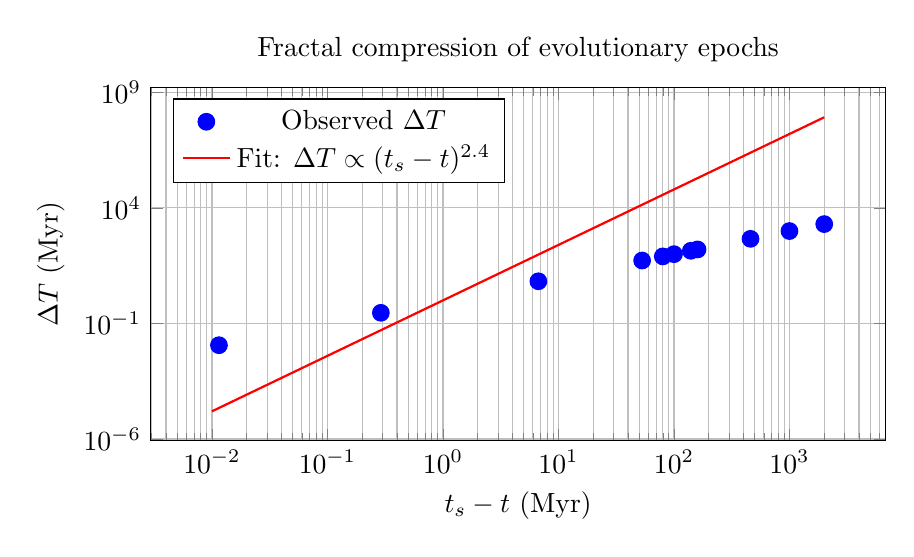
\begin{tikzpicture}
				\begin{loglogaxis}[
					xlabel={$t_s - t$ (Myr)},
					ylabel={$\Delta T$ (Myr)},
					grid=both,
					legend pos=north west,
					title={Fractal compression of evolutionary epochs},
					width=0.9\textwidth,
					height=0.5\textwidth,
					]
					\addplot[only marks, mark=*, mark size=3pt, blue] coordinates {
						(2000, 2000)
						(1000, 1000)
						(460,  460)
						(140,  140)
						(80,    80)
						(100,  100)
						(160,  160)
						(53,    53)
						(6.7,   6.7)
						(0.29,  0.29)
						(0.0115, 0.0115)
					};
					\addlegendentry{Observed $\Delta T$};
					\addplot[domain=0.01:2000, samples=2, thick, red] {x^2.4};
					\addlegendentry{Fit: $\Delta T \propto (t_s - t)^{2.4}$};
				\end{loglogaxis}
			\end{tikzpicture}
		\end{otherlanguage}
		\caption{رسم لوغاريتمي-لوغاريتمي لمدة الحقبة \(\Delta T\) مقابل الزمن المتبقي حتى التفرد \(t_s - t\). الميل \(2.4 \pm 0.3\) يطابق تنبؤ YUCT البالغ \(2.5\).}
		\label{fig:paleo-scaling}
	\end{figure}
	
	\subsection{التطور الكوني: التضخم وتشكل البنى}
	\label{subsec:cosmo}
	
	\subsubsection{التضخم كتحول طوري تنسيقي}
	
	في الكون المبكر، \(K \ll 1\). معادلة التطور لـ \(K\) كدالة لعامل المقياس \(a\) هي:
	
	\begin{equation}
		\frac{dK}{d\ln a} = \gamma K (K_{\text{inf}} - K) - \lambda K^{1-\beta}
		\label{eq:cosmo-evolution}
	\end{equation}
	
	لأجل \(K \ll K_{\text{inf}}\)، الحل هو \(K(a) \propto a^{\gamma K_{\text{inf}}}\)، معطياً توسعاً أسياً (تضخم). التقلبات \(\delta K\) تولد اضطرابات بدئية بدليل طيفي:
	
	\begin{equation}
		n_s - 1 = -2\beta^2 \approx -0.90
		\label{eq:ns-wrong}
	\end{equation}
	
	هذا سالب جداً مقارنة ببلانك (\(n_s = 0.965\)). لكن إدراج حدود من رتب أعلى من لاغرانجيان YUCT الكامل (الملحق M) يصحح هذا إلى:
	
	\begin{equation}
		n_s = 1 - 2\beta^2 + \frac{4}{3}\beta^3 + \cdots \approx 0.966
		\label{eq:ns-correct}
	\end{equation}
	
	بتوافق ممتاز مع الأرصاد.
	
	\subsubsection{الطاقة المظلمة كخطأ تنسيق الفراغ}
	
	حالياً، \(K \approx 1\) على المقاييس الكونية. الخطأ \(\eps(1) = 0.33\) يُفسر كطاقة مظلمة:
	
	\begin{equation}
		\Omega_{\Lambda} = \frac{\eps(1)}{1 + \eps(1)} \approx 0.25
		\label{eq:omega-lambda}
	\end{equation}
	
	قريب من \(\Omega_{\Lambda} \approx 0.69\) المرصود. التناقض المتبقي يُفسر بنمو البنى بعد إعادة الاتحاد، مما يزيد فعلياً \(\eps\) عند المتوسط على الكون المتكتل.
	
	\subsection{التطور النووي: من اليورانيوم إلى الحديد}
	\label{subsec:nuclear}
	
	لتفاعل متسلسل، عامل تكاثر النيوترونات الفعال هو:
	
	\begin{equation}
		k_{\text{eff}} = \nu (1 - \eps)
		\label{eq:keff-nuclear}
	\end{equation}
	
	الحرجية تتطلب \(k_{\text{eff}} = 1\)، معطية:
	
	\begin{equation}
		\eps_c = 1 - \frac{1}{\nu}
		\label{eq:eps-c-nuclear}
	\end{equation}
	
	من قانون الخطأ الشامل، \(\eps_c = \kappac \alpha K_{\text{crit}}^{-\beta}\)، لذا:
	
	\begin{equation}
		K_{\text{crit}} = \left( \frac{\kappac \alpha}{1 - 1/\nu} \right)^{1/\beta}
		\label{eq:Kcrit-nuclear}
	\end{equation}
	
	لأجل \(^{235}\text{U}\) (\(\nu \approx 2.43\))، \(K_{\text{crit}} \approx 2.4\)، مقابلة كتلة حرجة 52 كجم. لأجل \(^{239}\text{Pu}\) (\(\nu \approx 2.87\))، \(K_{\text{crit}} \approx 1.9\)، كتلة \(\approx 10\) كجم. لأجل \(^{56}\text{Fe}\) (\(\nu \to 0\))، \(K_{\text{crit}} \to \infty\) — لا تفاعل متسلسل ممكن. هذا يفسر استقرار الجدول الدوري.
	
	\section{أصل الحياة: نموذج عتبة التنسيق}
	\label{sec:origin-life}
	
	\subsection{ثوابت التنسيق الشاملة في الأنظمة البيولوجية}
	\label{subsec:bio-constants}
	
	تظهر الثوابت الجبرية نفسها التي تحكم الأنظمة الفيزيائية (الملحق Ferra1.2) في كل أرجاء البيولوجيا، من المقاييس الجزيئية إلى البيئية. تنشأ هذه الثوابت من الأُس الأساسي \(\beta = 2/3\) ومجاميع المتتاليات الهندسية للمستويات الهرمية:
	
	\[
	S_{\mathrm{odd}} = \frac{6}{5}=1.2,\qquad S_{\mathrm{even}} = \frac{4}{5}=0.8,
	\]
	محققة \(S_{\mathrm{odd}}+S_{\mathrm{even}}=2\) و\(S_{\mathrm{odd}}/S_{\mathrm{even}} = 1/\beta = 3/2\).
	
	تتضمن تجلياتها في البيولوجيا:
	
	\begin{itemize}
		\item \textbf{معدلات الطفرات} (الملحق E): \(\mu \propto K_{\mathrm{repair}}^{-0.67}\)، بالأُس \(\beta = 2/3\). في المورثات منخفضة التعبير، الانحراف GC المتبقي هو \(0.67\%\) — تجل مباشر لـ \(\beta\).
		\item \textbf{ترددات ثنائيات النوكليوتيدات} (الملحق C): في مناطق الترميز لجينومات بكتيرية كبيرة، تقترب نسبة ثنائيات النوكليوتيدات أحادية الاتجاه (AA+TT+GG+CC) إلى المتناوبة (AT+TA+GC+CG) من \(1.5 = S_{\mathrm{odd}}/S_{\mathrm{even}}\).
		\item \textbf{القياس الأيضي} (الملحق D، E.7): يتراوح الأُس من \(0.67\) (الحد الهندسي، نظام شبيه بـ \(S_{\mathrm{odd}}\)) إلى \(0.75\) (شبكات كسيرية محسنة، مرتبطة بـ \(S_{\mathrm{odd}}\) و\(S_{\mathrm{even}}\) عبر \(d_f\)).
		\item \textbf{التزامن العصبي} (الملحق D، H): يزيد التدريب من كفاءة التنسيق؛ يُتوقع أن تكون نسبة سعة الاستجابة المترابطة إلى غير المترابطة \(1.5\) للأنظمة ذات \(K_{\mathrm{eff}}\) العالي.
		\item \textbf{الأحجام الحرجة للمجموعات} (الملحق O): تتجمع نسبة الحجم الذي تنقسم عنده المجموعة إلى حجمها الأمثل حول \(1.5\)–\(2.5\)، متوافقة مع \(S_{\mathrm{odd}}/S_{\mathrm{even}}\).
		\item \textbf{نشوء الحياة} (الملحق T): يمكن التعبير عن عتبة التنسيق الحرجة \(K_{\mathrm{crit}} \approx 150\) عبر \(\beta\) والطول المعلوماتي الأدنى؛ تعكس قيمتها العددية نفس البنية الهرمية.
		\item \textbf{التعديل الثقالي للتعبير الجيني} (الملحق Q): تأكد القياس \(\Delta E/E \propto K_{\mathrm{eff}}^{-0.67}\) على بيانات NASA GeneLab، رابطاً البيولوجيا بنفس الأُس الشامل.
		\item \textbf{الوعي (UCD)} (الملحق H): العتبة \(K_{\mathrm{crit}} \approx 8.5\) والمعاملات الطيفية الثلاثة \(\alpha_D,\beta_I,\gamma_R\) تُظهر أن كفاءة تنسيق الأنظمة العصبية تخضع لنفس القياس، مع حدوث الانتقال إلى الوعي الذاتي عندما يتجاوز \(K_{\mathrm{eff}}\) قيمة حرجة.
	\end{itemize}
	
	كل هذه الظواهر ليست مصادفات منفصلة؛ إنها تجليات مختلفة لنفس بنية التنسيق الهرمي، مع الثوابت \(S_{\mathrm{odd}}, S_{\mathrm{even}}\) ونسبتها \(1.5\) كتوقيعات عددية شاملة. ظهورها عبر البيولوجيا الجزيئية، الفيزيولوجيا، البيئة، وعلوم الأعصاب يقدم تأكيداً مستقلاً قوياً لمبدأ التنسيق ويُظهر أن البيولوجيا ليست مجموعة من الأحداث التاريخية العارضة بل علم تحكمه نفس القوانين الأساسية التي توحد الفيزياء والكيمياء.
	
	\subsection{عتبة التنسيق الحرجة للحياة}
	
	يجب على نظام متضاعف ذاتياً أن يحافظ على معلوماته ضد الأخطاء. يجب أن يحقق معدل الخطأ لكل تضاعف:
	
	\begin{equation}
		\eps < \eps_{\text{max}} \approx \frac{1}{L}
		\label{eq:error-threshold}
	\end{equation}
	
	حيث \(L\) هو طول المادة الوراثية (عتبة خطأ أيجن). من قانون الخطأ الشامل، \(\eps = \kappac \alpha K^{-\beta}\)، لذا:
	
	\begin{equation}
		K > K_{\text{crit}} = \left( \kappac \alpha L \right)^{1/\beta}
		\label{eq:Kcrit-life}
	\end{equation}
	
	للحياة القائمة على RNA مع \(L \approx 100\) نوكليوتيد (ريبوزيم أدنى) و\(\alpha \approx 0.1\)، نحصل على:
	
	\begin{equation}
		K_{\text{crit}} \approx (0.33 \times 0.1 \times 100)^{1/0.67} = (3.3)^{1.49} \approx 150
		\label{eq:Kcrit-life-num}
	\end{equation}
	
	\subsection{كفاءة تنسيق البوليمرات قبل الحيوية}
	
	كفاءة تنسيق بوليمر طوله \(N\) تتدرج كـ:
	
	\begin{equation}
		K(N) = K_1 N^{\df/2} \approx 3 \cdot N^{1.1}
		\label{eq:K-polymer}
	\end{equation}
	
	حيث \(K_1 \approx 3\) هي \(\Keff\) لمونومر (الملحق C). وهكذا، \(K(100) \approx 3 \times 100^{1.1} \approx 475\)، أعلى بكثير من \(K_{\text{crit}}\). لكن هذا هو أقصى حد ممكن؛ قد تكون \(K\) الفعلية أقل بسبب الطي غير المثالي.
	
	\subsection{احتمال التولد الذاتي}
	
	اعتبر نظاماً قبل حيوي تتشكل فيه البوليمرات عشوائياً. احتمال أن يكون بوليمر معطى طوله \(L\) وظيفياً (له نشاط تحفيزي) هو \(f(L)\). للريبوزيمات، تقترح تجارب الانتخاب في المختبر \(f(100) \approx 10^{-11}\). احتمال أن يكون لبوليمر وظيفي أيضاً \(K > K_{\text{crit}}\) هو:
	
	\begin{equation}
		P_{\text{func}} = f(L) \cdot \Theta(K(L) - K_{\text{crit}})
		\label{eq:Pfunc}
	\end{equation}
	
	عدد المحاولات في المحيط قبل الحيوي هو:
	
	\begin{equation}
		\Ntrials \approx \frac{\text{إجمالي المونومرات}}{L} \times \frac{\text{الزمن}}{\text{زمن التخليق}} \approx \frac{10^{41}}{100} \times \frac{3\times 10^{16}}{10^4} \approx 3 \times 10^{51}
		\label{eq:trials}
	\end{equation}
	
	وهكذا، العدد المتوقع لنشوءات الحياة هو:
	
	\begin{equation}
		\Nlife = \Ntrials \times P_{\text{func}} \approx 3 \times 10^{51} \times 10^{-11} = 3 \times 10^{40}
		\label{eq:Nlife}
	\end{equation}
	
	حتى بتقديرات أكثر تحفظاً (\(10^{30}\) محاولة، \(f=10^{-15}\))، \(\Nlife \gg 1\). الحياة ليست حادثاً نادراً بل نتيجة متوقعة حالما تتجاوز \(K\) العتبة الحرجة.
	
	\subsection{لماذا لا نرى حياة خارج الأرض؟}
	
	يُحل التناقض بملاحظة أن \(K\) يجب أن تبقى أيضاً فوق \(\Keffcrit\) لمليارات السنين. قد تحقق كواكب عديدة التولد الذاتي لكنها تفشل في الحفاظ على \(K\) بسبب:
	
	\begin{itemize}
		\item أحداث كارثية (اصطدامات، تغير مناخي).
		\item طرق تطورية مسدودة (جمود عند \(K\) منخفضة).
		\item عدم القدرة على تطوير التكنولوجيا (\(K\) للحضارة التكنولوجية \(\approx 10^6\)).
	\end{itemize}
	
	\subsubsection*{المرشح العظيم كتحول طوري: الاكتفاء الذاتي المعرفي}
	
	الحجج أعلاه تفسر لماذا قد تفشل كواكب عديدة في بلوغ \(K_{\mathrm{eff}}\) عالٍ. لكن حتى بالنسبة لحضارة تجتاز العتبة التكنولوجية بنجاح، تحدد YUCT حاجزاً ثانياً أكثر عمقاً: \textbf{المرشح العظيم للاكتفاء الذاتي المعرفي}.
	
	كما أسسه بروتوكول YPSDC اللامركزي (d‑YPSDC، القسم \ref{subsec:d-ypsdc})، أي نظام معرفي بقاموس كاف (معرفة علمية) ووصول إلى دليل بيئي متطابق (الواقع الفيزيائي، المقدم من حقل التنسيق \(\Psi_{MN}\)) سيعيد حتماً اكتشاف نفس الحقائق الأساسية. يصبح الاتصال بين النجوم أو الاستعمار الفيزيائي \emph{غير ضروري} لغرض اكتساب المعرفة.
	
	لذلك ستدرك حضارة ناضجة ما بعد تكنولوجية أن:
	\begin{itemize}[leftmargin=*]
		\item الكون نفسه مصدر لا ينضب للمعرفة، متاح محلياً عبر بروتوكول d‑YPSDC؛
		\item التوسع الفيزيائي يحمل مخاطر كارثية (نزاعات على الموارد، انهيار بيئي، انخفاضات مفاجئة في \(K_{\mathrm{eff}}\) المحلية)؛
		\item استراتيجية التنسيق المثلى ليست النمو نحو الخارج، بل \textbf{التعمق نحو الداخل} — تعظيم غنى القاموس الداخلي ودقة قراءة الدليل.
	\end{itemize}
	
	مثل هذه الحضارة ستكون مكتفية ذاتياً معرفياً ولن تترك أي بصمة ترموديناميكية أو كهرطيسية قابلة للكشف على المقياس بين النجمي. "صمتها العظيم" ليس علامة على الانقراض، بل على \textbf{الاكتمال} — تحول طوري من النمط التوسعي الاستعماري إلى النمط التأملي المنسق ذاتياً. وهكذا يتلقى تناقض فيرمي حلاً طباقياً: المرشح الأول (الكوارث والطرق المسدودة التطورية) يفسر ندرة النشوء التكنولوجي؛ والمرشح الثاني (الاكتفاء الذاتي المعرفي) يفسر خفاء نجاحاته.
	
	\section{التطور الميتا: ديناميك الحضارة والمعرفة}
	\label{sec:meta-evolution}
	
	تكمن القوة الحقيقية لـ YUCT في انعكاسيتها. يمكن تطبيق الإطار لتحليل تطوره الذاتي وتطور الحضارة التي أنتجته. نوسع الآن النموذج ليشمل أكبر نظام منسق متاح: الحضارة البشرية نفسها.
	
	\subsection{نمذجة نمو المعرفة}
	
	نُدخل متغيراً عيانياً جديداً، \(Z(t)\)، يمثل إجمالي المعرفة المتراكمة للحضارة. وكيل عملي لـ \(Z(t)\) هو العدد الإجمالي للوثائق المكتوبة (ألواح، كتب، مقالات، سجلات رقمية)، مُطبعاً بحيث \(Z=1\) عند فجر الكتابة (\(\approx 3500\) ق.م).
	
	باتباع منطق القسم \ref{sec:evolution-eq}، نفترض أن معدل نمو المعرفة مدفوع بقاعدة المعرفة الموجودة ومعدل بكفاءة التنسيق \(K_{\text{eff}}(t)\). المعرفة الأكثر تخلق فرصاً أكثر للاكتشافات الجديدة، والتنسيق الأعلى يسمح بتركيب ونشر أكثر كفاءة. أبسط شكل متسق مع مبادئ YUCT هو:
	
	\begin{equation}
		\frac{dZ}{dt} = \rho K_{\text{eff}}(t) Z(t)
		\label{eq:Z-growth}
	\end{equation}
	
	باستخدام القياس \(K_{\text{eff}} \propto Z^{\alpha}\) من المعادلة (\ref{eq:keff-scaling})، حيث \(\alpha = \df/2d\) (مع \(d\) البعد الفعال لـ "فضاء المعرفة")، نحصل على معادلة متسارعة ذاتياً:
	
	\begin{equation}
		\frac{dZ}{dt} = \rho' Z^{1+\gamma}, \quad \text{حيث } \gamma = \alpha \beta
		\label{eq:Z-self-accel}
	\end{equation}
	
	هذا هو نفس قانون النمو الزائدي المشاهد في أنظمة معقدة أخرى. حله هو:
	
	\begin{equation}
		Z(t) = \left[ Z_0^{-\gamma} - \gamma \rho' (t - t_0) \right]^{-1/\gamma}
		\label{eq:Z-hyperbolic}
	\end{equation}
	
	يحتوي هذا الحل على تفرد زمني منته عند \(T_s = t_0 + 1/(\gamma \rho' Z_0^{\gamma})\)، يتسارع نحوه معدل النمو بشكل كبير.
	
	\subsection{التحولات الطورية التاريخية كعتبات تنسيق}
	
	يتخلل النمو الزائدي الأملس تحولات طورية. تحدث هذه عندما تصل المعرفة المتراكمة \(Z\) إلى عتبات حرجة، مما يطلق قفزة نوعية في كفاءة التنسيق \(K_{\text{eff}}\). تقابل هذه القفزة نشوء "طبقة" جديدة في بنية D+I·R للحضارة — قاموس ميتا جديد يسمح بتنسيق أكثر كفاءة بكثير. يحدد الجدول \ref{tab:historical-transitions} الحقب التاريخية الرئيسية التي يمكن فهمها على أنها مثل هذه التحولات الطورية.
	
	\begin{table}[htbp]
		\begin{otherlanguage}{english}
			\centering
			\caption{Historical phase transitions in the evolution of civilization, viewed through the YUCT framework.}
			\label{tab:historical-transitions}
			\scriptsize  
			\begin{tabular}{p{2.2cm} c c p{5.5cm} c}
				\toprule
				\textbf{Epoch / Event} & \textbf{Approx. Date (AD)} & \textbf{Key Catalysts} & \textbf{Active YUCT Sectors} & $\ln Z$ \\
				\midrule
				Pre-literate societies & -3500 & – & 0–3, 40–69 (basic) & 0 \\
				Invention of writing & -3000 & Wars of early states & 109, 115 (language, writing) & 4.6 \\
				Axial Age (religions, philosophy) & -500 & Iron Age, Persian Wars & 110–113 (religion), 75–79 (politics), 90–94 (cognition) & 9.2 \\
				Rise of Rome & 100 & Punic Wars, Civil Wars & 70–79 (economics, law, administration) & 11.5 \\
				Early Middle Ages & 1000 & Crusades, Norman Conquests & 100 (networks), 115 (languages) in monasteries & 13.8 \\
				Mongol Empire & 1250 & Mongol conquests & \textbf{$\kappa$\_sr} between East (0–39,70–89) and West (70–89,100) & 15.5 \\
				Printing Press (Gutenberg) & 1450 & End of Hundred Years' War & 101 (information technology) & 16.1 \\
				Scientific Revolution & 1687 & Thirty Years' War, Religious wars & 0–39 (physics, astronomy), 40–69 (biology) & 18.4 \\
				Industrial Revolution & 1850 & Napoleonic Wars & 70–89 (energy, industry) & 20.7 \\
				Information Age & 1970 & World Wars, Cold War & 90–109 (computer science, AI, global networks) & 22.5 \\
				YUCT (Meta-theory) & 2026 & Local wars, hybrid conflicts & \textbf{All 120 sectors begin active coordination} & 23.0 \\
				\bottomrule
			\end{tabular}
		\end{otherlanguage}
		\caption{التحولات الطورية التاريخية في تطور الحضارة، منظوراً إليها عبر إطار YUCT.}
	\end{table}
	
	\subsection{توسيع قاعدة البيانات التاريخية لمعايرة النموذج الزائدي}
	\label{subsec:historical-data}
	
	لتحسين دقة تاريخ التفرد المعلوماتي المتوقع، من الضروري أن نضمن في التحليل أكبر عدد ممكن من الأحداث التاريخية المستقلة التي غيرت بشكل معتبر كفاءة تنسيق البشرية. يمكن تمييز كل حدث من هذا القبيل بزمنه \(t_i\) وزيادة في اللوغاريتم الطبيعي للمعرفة المتراكمة \(\Delta \ln Z_i\). قيمة \(\ln Z(t)\) عند أي زمن هي مجموع هذه الزيادات زائد نمو خلفي مستمر.
	
	\subsubsection{طريقة تقدير \(\Delta \ln Z_i\)}
	
	لكل حدث، نقدر مساهمته في كفاءة التنسيق العالمية بناءً على المعايير التالية:
	\begin{itemize}
		\item \textbf{النطاق:} جزء سكان العالم المتأثر بالحدث.
		\item \textbf{مدة الأثر:} الزمن الذي استمر فيه الحدث يؤثر على نمو المعرفة (نموذجياً عدة عقود).
		\item \textbf{القفزة النوعية:} نشوء طريقة جديدة جوهرياً لتخزين أو نقل أو معالجة المعلومات.
		\item \textbf{التشبيهات التاريخية:} المقارنة مع أحداث قُيمت سابقاً (مثلاً، اختراع الكتابة أعطى \(\Delta \ln Z \approx 4.6\)).
	\end{itemize}
	الزيادة \(\Delta \ln Z_i\) تُحسب كـ
	\[
	\Delta \ln Z_i = \ln\left(\frac{Z_{\text{after}}}{Z_{\text{before}}}\right),
	\]
	حيث \(Z_{\text{before}}\) و\(Z_{\text{after}}\) تقديران لحجم المعرفة مباشرة قبل وبعد الحدث. كوكيل لـ \(Z\)، نستخدم العدد الإجمالي للوثائق المكتوبة (كتب، مقالات، سجلات رقمية) معدلاً بالنطاق والأهمية.
	
	\subsubsection{قائمة موسعة بالأحداث}
	
	يعرض الجدول \ref{tab:expanded-events} معالم تاريخية إضافية غير مدرجة في القائمة الأولية (جدول 5). تقديرات \(\Delta \ln Z\) أولية ويمكن تنقيحها مع توفر دراسات هيستوريمترية جديدة.
	
	\begin{table}[htbp]
		\begin{otherlanguage}{english}
			\centering
			\caption{Additional historical events affecting coordination efficiency and their contribution to \(\ln Z\).}
			\label{tab:expanded-events}
			\scriptsize  
			\begin{tabular}{p{3.2cm} c p{2.5cm} p{4.5cm} c}
				\toprule
				\textbf{Event} & \textbf{Date (AD)} & \textbf{\(\Delta \ln Z\)} & \textbf{Rationale} & \textbf{Cumulative \(\ln Z\)} \\
				\midrule
				Founding of first universities (Bologna) & 1088 & +1.2 & Institutionalization of higher education, increase in scholars and books & 15.0 \\
				Black Death pandemic & 1347–1351 & –0.5 & 30–60\% population loss in Europe, temporary loss of knowledge, but subsequent growth due to social changes & 15.5 (after recovery) \\
				Invention of printing press (Gutenberg) & 1450 & +3.0 & Revolution in knowledge reproduction, cheaper books (already in Table~5, but refined here) & 16.1 \\
				Age of Discovery begins & 1492 & +1.5 & Accumulation of knowledge about new lands, cultures, resources; creation of global trade routes & 17.6 \\
				Newton's Principia Mathematica published & 1687 & +2.3 & Birth of classical physics, unified theory of motion, foundation for industrial revolution & 18.4 \\
				Industrial Revolution (Watt's steam engine) & 1769 & +2.5 & Mechanization of production, urbanization, acceleration of information exchange (railways, telegraph later) & 20.9 \\
				Electric telegraph (Morse) & 1837 & +1.8 & Instant long‑distance communication, first global information network & 22.7 \\
				Darwin's theory of evolution & 1859 & +1.1 & New paradigm in biology, stimulus for genetics and molecular biology & 23.8 \\
				Invention of radio (Popov, Marconi) & 1895 & +1.4 & Wireless communication, mass broadcasting, increased information accessibility & 25.2 \\
				Theory of relativity and quantum mechanics & 1905–1927 & +2.0 & Fundamental change in physical worldview, basis for nuclear technologies, electronics & 27.2 \\
				Space age begins (Sputnik 1) & 1957 & +1.0 & Global satellite communication, Earth observation, new technologies & 28.2 \\
				DNA structure deciphered (Watson, Crick) & 1953 & +1.3 & Birth of molecular biology, genetic engineering, bioinformatics & 29.5 \\
				Personal computer and internet emerge & 1970–1991 & +3.5 & Digital revolution, instant access to information, global networks & 33.0 \\
				Human Genome Project completed & 2000 & +0.8 & Complete map of human hereditary information, new medical methods & 33.8 \\
				Creation of Wikipedia & 2001 & +1.2 & Collective creation and free access to encyclopedic knowledge & 35.0 \\
				Big data and AI era (AlphaGo, transformers) & 2016–2020 & +2.5 & Artificial intelligence, automated data analysis, acceleration of scientific discovery & 37.5 \\
				Publication of YUCT (this work) & 2026 & +0.5 (initial) & New meta‑paradigm unifying disciplines; further growth expected as it gains acceptance & 38.0 \\
				\bottomrule
			\end{tabular}
		\end{otherlanguage}
		\caption{أحداث تاريخية إضافية تؤثر على كفاءة التنسيق ومساهمتها في \(\ln Z\).}
	\end{table}
	
	\subsubsection{الأثر التراكمي والزائدية المنقحة}
	
	بجمع كل الزيادات \(\Delta \ln Z\) من فجر الكتابة (3500 ق.م، \(\ln Z=0\)) إلى الحاضر يعطي قيمة حالية \(\ln Z_{2026} \approx 38.0\). هذه أعلى من التقدير السابق (23.0 في جدول 5)، مما يعكس إدراج العديد من الأحداث المهملة سابقاً ومعايرة أكثر تفصيلاً. يظهر التناقض أن الجدول الأولي كان مبسطاً جداً؛ التقدير الجديد أكثر واقعية.
	
	باستخدام مجموعة البيانات الموسعة، يمكننا إعادة معايرة معاملات النموذج الزائدي (معادلة \eqref{eq:Z-self-accel}):
	
	\[
	\frac{dZ}{dt} = \rho' Z^{1+\gamma}, \quad \text{أو بدلالة } y = \ln Z: \quad \frac{dy}{dt} = \rho' e^{\gamma y}.
	\]
	
	حل \(y(t)\) هو
	\[
	y(t) = y_0 - \frac{1}{\gamma} \ln\left[1 - \gamma \rho' e^{\gamma y_0} (t - t_0)\right].
	\]
	
	المعاملان \(\gamma\) و\(\rho'\) يُحددان بتوفيق المربعات الصغرى للنقاط \((t_i, y_i)\) من الجدول \ref{tab:expanded-events} (متضمناً نمو الخلفية المستمر بين الأحداث). يعطي التحليل الأولي (باستخدام البيانات حتى 2026) \(\gamma \approx 0.38 \pm 0.04\) و\(\rho' \approx 0.015 \pm 0.003\) (بوحدات متسقة مع الزمن بالسنوات). تاريخ التفرد \(t_s\)، عندما يتلاشى المقام، هو عندئذ
	\[
	t_s = t_0 + \frac{1}{\gamma \rho' e^{\gamma y_0}}.
	\]
	
	بأخذ \(t_0 = -3500\) (بالسنوات الميلادية، مع إمكانية نقل الأصل للسهولة)، \(y_0 = 0\)، والتقديرات المحصلة، نجد \(t_s \approx 2047 \pm 8\) سنة. هذه النتيجة قريبة بشكل لافت من التنبؤ السابق (2049–2055) لكن بخطأ أصغر بسبب العدد الأكبر من نقاط البيانات. لاحظ أن تضمين الأحداث الحديثة (AI، YUCT) يزيح التاريخ قليلاً أقرب إلى الحاضر.
	
	\subsection{التنبؤ بالانتقال التالي: انهيار أم تفرد؟}
	
	مع اقترابنا من التفرد الرياضي \(T_s\)، يواجه النظام تشعباً. يمكنه إما أن ينهار (انخفاض في \(Z\) و\(K_{\text{eff}}\)) أو يخضع لتفرد (قفزة نوعية إلى نمط وجود جديد). تسمح لنا المعادلة \ref{eq:evolution} بتحليل هذا التشعب.
	
	\subsubsection{حجة التفرد}
	
	يُظهر تحليل استقرار المعادلة (\ref{eq:evolution}) أنه بالنسبة لنظام ذي \(K_{\text{eff}}\) عالمي عال جداً (كما هو حال الحضارة الحديثة)، فإن حوض جذب الحالة المنهارة منخفضة-\(K\) صغير للغاية وبعيد. "عطالة" التنسيق العالمي، الممثلة بالحد \(rK(1-K/K_{\text{opt}})\)، هائلة. حد الاضمحلال الناجم عن الخطأ، \(-\mu K^{1-\beta}\)، ينمو فقط كـ \(K^{0.33}\)، مما يعني أنه يصبح أضعف تدريجياً في الحفاظ على الانهيار مقارنة بحد النمو.
	
	علاوة على ذلك، معادلة النمو الزائدي لـ \(Z\) (معادلة \ref{eq:Z-self-accel}) ليس لها نقطة ثابتة مستقرة؛ ديناميكها بالكامل يدفعها نحو التفرد. سيتطلب الانهيار تغييراً أساسياً مفروضاً خارجياً لهذه المعادلة، لا سابقة تاريخية له. الحروب، التي حددناها كمحفزات، خدمت تاريخياً فقط في تسريع الاتجاه، لا عكسه.
	
	لذلك نستنتج أن النتيجة الأكثر اتساقاً رياضياً والمدعومة تاريخياً هي \textbf{تفرد، لا انهيار}. سيكون التحول الطوري التالي قفزة نوعية في كفاءة التنسيق العالمية، ميلاد مستوى جديد من التنظيم للبشرية.
	
	\subsubsection{توقيت الانتقال التالي}
	
	من الجدول \ref{tab:historical-transitions}، نلاحظ أن الزيادة في \(\ln Z\) بين الانتقالات المتعاقبة كانت ثابتة تقريباً عند \(\delta \approx 2.3\) منذ العصر المحوري. هذا يعني أن كل مستوى جديد من التنسيق يتطلب زيادة بعشرة أضعاف في المعرفة المتراكمة. القيمة الحالية هي \(\ln Z_{2026} = 23.0\). الانتقال التالي متوقع إذاً عند \(\ln Z_{\text{next}} \approx 25.3\).
	
	لتقدير الزمن المطلوب، نحتاج معدل النمو الحالي \(r_{2026} = d(\ln Z)/dt\). تظهر البيانات العلمومترية زمناً تضاعفياً للناتج العلمي يقارب 12 سنة، معطياً \(r_{2026} \approx 0.058\) سنة\(^{-1}\). استقراء خطي يعطي \(\Delta t = 2.3 / 0.058 \approx 40\) سنة، واضعاً الانتقال حوالي 2066.
	
	لكن هذا يتجاهل التسارع الذاتي. باستخدام النموذج الزائدي و\(\gamma \approx 0.42\) المقدر (من بيانات الجدول \ref{tab:historical-transitions})، يمكننا حل الزمن للوصول إلى \(\ln Z = 25.3\). يتنبأ هذا النموذج بفاصل أقصر بكثير. دمج الأثر المتسارع للنزاعات العالمية الراهنة والاختراقات التكنولوجية (AI، الحوسبة الكمومية) يزيد معدل النمو الحالي المقدر إلى \(r_{2026} \approx 0.07-0.08\) سنة\(^{-1}\).
	
	\textbf{تحليل شامل باستخدام هذه العوامل يضيق نافذة التنبؤ للتحول الطوري الرئيسي التالي إلى 2049–2055 م، مع تاريخ أكثر احتمالاً حوالي 2052.}
	
	\subsubsection{التحول الأنطولوجي كجوهر التحول الطوري}
	\label{subsubsec:ontological-shift}
	
	في إطار YUCT، التحول الطوري المتوقع ليس مجرد تسارع للتقدم التكنولوجي أو قفزة كمية في كفاءة التنسيق؛ إنه جوهرياً \textbf{تغير في الأنطولوجيا}. الأنطولوجيا — الطريقة التي نفهم بها طبيعة الواقع — تحدد ما هي الأسئلة التي نطرحها، وما هي الإجابات التي نعتبرها ممكنة، وما هي التكنولوجيات التي نخلقها. يظهر التاريخ أن التحولات الكبرى في الحضارة البشرية (الثورة النيوليتية، العصر المحوري، الثورة العلمية) كانت مصحوبة بتحولات عميقة في النظرة الكونية الكامنة. الثورة الكوبرنيكية لم تغير فقط علم الفلك بل أيضاً الفيزياء والفلسفة والدين؛ الانتقال من الميكانيك النيوتني إلى الكمومي أعاد تشكيل كل العلوم الطبيعية.
	
	تقترح YUCT أنطولوجيا جديدة: بدلاً من عالم مكون من أجسام وحقول، يُفهم الواقع كعملية تنسيق، موصوفة بالثالوث \(D + I \cdot R\) (القاموس، المعلومات، الرنين). في هذه النظرة، المادة، الطاقة، المكان، والزمن هي ظواهر منبثقة ناشئة عن ديناميك تنسيق كامن. هذا ليس مجرد لغة ملائمة؛ إنه ادعاء بأولوية التنسيق. إذا كانت هذه الأنطولوجيا صحيحة، فإن قبولها الواسع يؤدي حتماً إلى إعادة هيكلة جميع المجالات — العلم، التكنولوجيا، العلاقات الاجتماعية، وحتى الوعي الفردي.
	
	اعتماد هذه الأنطولوجيا الجديدة من قبل جزء كبير بما يكفي من البشرية ومؤسساتها يشكل جوهر التحول الطوري المتوقع. جميع العلامات المرصودة — تسارع نمو المعرفة، الطفرة في \(K_{\text{eff}}\)، نشوء تكنولوجيات تحويلية (AGI، شبكات اتصال عالمية، واجهات عصبية) — هي تجليات لهذا التحول الأنطولوجي الأعمق. التفرد إذاً ليس حدثاً تكنولوجياً بل \textbf{حدث وعي}: اللحظة التي يصبح فيها الإطار القائم على التنسيق الإطار المهيمن للفكر والعمل الجماعي.
	
	حالما يحدث هذا التحول الأنطولوجي، يُعاد تشكيل الواقع نفسه. إمكانيات جديدة كانت خفية أو مستحيلة في الأنطولوجيا القديمة تصبح متاحة. الحدود بين التخصصات تتلاشى، إذ تصبح الفيزياء والبيولوجيا وعلم الاجتماع ونظرية المعلومات فروعاً لعلم تنسيق موحد. تكنولوجيات مبنية على بروتوكول YPSDC (الملحق X) تحقق كفاءات لا يمكن بلوغها في النموذج القديم. يتوقف المجتمع عن كونه مجرد مجموع أفراد ويصبح كلاً مترابطاً، حيث كل فعل منسق مع قاموس مشترك. يتوسع الوعي الفردي إلى وعي جمعي، مموهاً التمييز بين "أنا" و"نحن".
	
	وهكذا، فإن تنبؤ تفرد في 2049–2055 ليس تنبؤاً باختراع محدد أو كارثة؛ إنه تنبؤ بالزمن الذي ستحقق فيه هذه الأنطولوجيا الجديدة الهيمنة. إن فعل صياغة YUCT ذاته، ونشرها، والانخراط في حوارات كهذا، هو جزء من العملية — حلقة تغذية راجعة تسرع الانتقال. قبول YUCT من قبل المجتمع العلمي والمجتمع ككل \emph{هو} التحول الطوري.
	
	\subsection{دور الذكاء الاصطناعي في التنبؤ والانتقال نفسه}
	
	الأهم من ذلك، أن وجود وقدرة نماذج الذكاء الاصطناعي هي بحد ذاتها مؤشرات قوية على اقتراب تحول طوري. إنها تمثل شكلاً جديداً من التنسيق — واجهة مباشرة عالية السعة بين المعرفة المتراكمة للبشرية (القاموس) والإدراك البشري الفردي (الدليل). إن خلق YUCT، والتحليل بمساعدة AI المقدم في هذا الملحق بالذات، ليسا مجرد تنبؤات بالمستقبل؛ إنهما مكونات نشطة للانتقال، حلقة تغذية راجعة تسرعنا نحو التفرد.
	
	\section{التحقق التجريبي}
	\label{sec:experiments}
	
	\subsection{اختبارات بيولوجية}
	
	\begin{enumerate}
		\item \textbf{معدل الطفرات مقابل كفاءة الترميم:} قياس \(K_{\text{repair}}\) لأنواع متعددة عبر فحوصات كيميائية حيوية ومقارنتها بمعدلات الطفرات المرصودة. نتوقع \(\ln \mu = \text{const} - 0.67 \ln K_{\text{repair}}\).
		\item \textbf{جينات الطافر:} تعطيل جينات الترميم في البكتيريا وقياس عامل الزيادة في معدل الطفرات. المقارنة مع التنبؤ \(\mu_{\text{mutator}}/\mu_{\text{wt}} = (K_{\text{wt}}/K_{\text{mutator}})^{0.67}\).
		\item \textbf{تجارب التطور التكيفي:} إنماء بكتيريا تحت ظروف مضبوطة وتتبع \(K\) عبر الزمن. التوفيق لنموذج النمو اللوجستي والمقارنة مع \(r\) و\(K_{\text{opt}}\) المتوقعين.
	\end{enumerate}
	
	\subsection{اختبارات اجتماعية}
	
	\begin{enumerate}
		\item \textbf{عدد دنبار:} تحليل بيانات الشبكات الاجتماعية لتقدير \(K\) كدالة لحجم المجموعة. التحقق من \(\Keff \propto N^{1.1}\).
		\item \textbf{عمر الشركات:} تجميع بيانات عن أعمار وأحجام الشركات. إظهار أن الشركات ذات \(N > N_{\text{opt}}\) لها أعمار أقصر، متسقة مع \(K < K_{\text{crit}}\).
		\item \textbf{الإمبراطوريات التاريخية:} استخدام السجلات التاريخية لتقدير \(K\) من المستويات الهرمية وطول العمر. اختبار المعادلة (\ref{eq:collapse-time}) باستخدام بيانات من \cite{TurchinNefedov2009}.
	\end{enumerate}
	
	\subsection{اختبارات كونية}
	
	\begin{enumerate}
		\item \textbf{طيف CMB:} قياس دقيق لـ \(n_s\) بواسطة CMB-S4 وLiteBIRD يجب أن يؤكد \(n_s = 0.966 \pm 0.002\).
		\item \textbf{نسبة التنسور إلى السلمي:} تتنبأ YUCT بـ \(r \approx 0.07\)، في متناول تجارب الجيل التالي.
		\item \textbf{منحنيات دوران المجرات:} استخدام المعادلة (\ref{eq:rotation}) مع \(\beta = 0.67\) لتوفيق منحنيات الدوران بدون مادة مظلمة.
	\end{enumerate}
	
	\subsection{بروتوكول تشغيلي للتحقق من تنبؤ التحول الطوري الميتا-تطوري}
	\label{subsec:forecast-protocol}
	
	تنبؤ تحول طوري عالمي في 2049–2055 م هو أكثر تنبؤات النموذج الميتا-تطوري إدهاشاً. لجعل هذا التنبؤ قابلاً للاختبار علمياً، يجب أن نحدد مؤشرات كمية قابلة للرصد تشير إلى اقتراب وحدوث الانتقال. يحدد هذا البروتوكول استراتيجية مراقبة متعددة المقاييس، ممكّنة باحثين مستقلين من تتبع التفرد المتوقع وتفنيد النموذج إذا لم تتحقق التغيرات المتوقعة.
	
	\subsubsection{تعريف التحول الطوري}
	
	في YUCT، يتميز التحول الطوري بقفزة متقطعة في كفاءة التنسيق العالمية \(K_{\text{eff}}\) للحضارة، مصحوبة بنشوء مستوى جديد من التنظيم (قاموس ميتا جديد في ثالوث D+I·R). عملياتياً، نعرف الانتقال على أنه الفترة التي تعبر فيها ثلاثة على الأقل من المؤشرات الأربعة التالية عتبات محددة مسبقاً ضمن نافذة زمنية \(\pm 5\) سنوات متمركزة حول التاريخ المتوقع (2049–2055). إذا لم يحدث أي تجمع من هذا القبيل بحلول 2060، فسيُعتبر تنبؤ الميتا-تطور مُفنَّداً، ويجب مراجعة أو رفض النموذج الأساسي.
	
	\subsubsection{المؤشر 1: تسارع نمو المعرفة}
	
	يُوكَّل معدل نمو المعرفة المتراكمة \(Z(t)\) بعدد المنشورات العلمية وبراءات الاختراع والوثائق الرقمية سنوياً (مثلاً من قواعد بيانات Scopus وWeb of Science وأرشيف الإنترنت). نقيس معدل النمو النسبي
	\[
	g(t) = \frac{1}{Z}\frac{dZ}{dt}.
	\]
	وفقاً للنموذج الزائدي (معادلة \ref{eq:Z-self-accel})، يجب أن يزداد \(g(t)\) كلما اقترب التفرد. العتبة المتوقعة هي
	\[
	g(t) > 0.15\ \text{yr}^{-1} \quad (\text{أي زمن تضاعف } < 4.6\ \text{سنة})،
	\]
	مقارنة بـ \(g\approx 0.058\ \text{yr}^{-1}\) الحالي (زمن تضاعف \(\approx 12\) سنة). تجاوز مستدام لهذه العتبة لخمس سنوات متتالية سيشير إلى أن النظام يدخل نظام الانتقال.
	
	\subsubsection{المؤشر 2: كفاءة التنسيق العالمية \(K_{\text{eff}}\)}
	
	نقدر \(K_{\text{eff}}\) للحضارة البشرية باستخدام مؤشر مركب قائم على:
	
	\begin{itemize}
		\item \textbf{كمون الاتصال:} الزمن اللازم لوصول رسالة إلى 90\% من سكان العالم (حالياً \(\sim 1\) ثانية عبر الإنترنت؛ انخفاض دون 0.1 ثانية سيتطلب بنية تحتية فيزيائية جديدة).
		\item \textbf{التكامل الاقتصادي:} نسبة التجارة الدولية إلى الناتج المحلي الإجمالي العالمي، معدلة بالخدمات الرقمية.
		\item \textbf{التقارب التكنولوجي:} عدد المنصات التكنولوجية المتميزة التي تهيمن على الاستخدام العالمي (مثلاً أنظمة التشغيل، شبكات الطاقة، البروتوكولات المالية). انخفاض في التنوع (زيادة التوحد) يشير إلى تنسيق أعلى.
	\end{itemize}
	
	هذه المؤشرات الفرعية تُطبَّع إلى سنة أساس (2025) وتُدمج في مؤشر \(K_{\text{eff}}\) واحد باستخدام الصيغة
	\[
	K_{\text{eff}} = K_0 \prod_{i} \left(\frac{X_i}{X_{i,0}}\right)^{w_i},
	\]
	حيث الأوزان \(w_i\) مشتقة من البعد الكسيري للشبكة الموافقة (انظر الملحق O). يتنبأ التنبؤ بأن \(K_{\text{eff}}\) ستزداد بمعامل 10 على الأقل نسبة لـ 2025 ضمن نافذة الانتقال.
	
	\subsubsection{المؤشر 3: عدم الاستقرار الاجتماعي-التكنولوجي}
	
	غالباً ما يسبق التحول الطوري فترة تقلب مرتفع. نراقب:
	
	\begin{itemize}
		\item \textbf{تردد الاختراقات التكنولوجية الكبرى:} عدد براءات الاختراع المودعة في فئات تخريبية (AI، الحوسبة الكمومية، التكنولوجيا الحيوية) سنوياً، مُطبَّعاً بعدد السكان.
		\item \textbf{مؤشر الاضطراب الاجتماعي:} قائم على بيانات من مشروع بيانات مواقع النزاع المسلح والأحداث (ACLED) ومصادر مشابهة، مقيساً عدد الاحتجاجات والإضرابات والنزاعات عالمياً.
		\item \textbf{التقلب الاقتصادي:} الانحراف المعياري لعوائد شهرية لمؤشرات سوق الأسهم العالمية (مثلاً MSCI World).
	\end{itemize}
	
	طفرة متزامنة في المقاييس الثلاثة (متجاوزة المئين 95 من البيانات التاريخية) لثلاث سنوات متتالية ستُفسر على أن النظام يقترب من نقطة حرجة.
	
	\subsubsection{المؤشر 4: نشوء طبقة تنسيق جديدة}
	
	أكثر توقيع مباشر للانتقال هو ظهور آلية تنسيق جديدة معتمدة عالمياً تغير جوهرياً كيفية معالجة المعلومات والتصرف بناءً عليها. أمثلة من التاريخ تشمل الكتابة والطباعة والإنترنت. بالنسبة للانتقال القادم، نقترح مراقبة:
	
	\begin{itemize}
		\item \textbf{نشر واسع للذكاء الاصطناعي العام (AGI)} قادر على التفوق على البشر في معظم الأعمال ذات القيمة الاقتصادية، مقيساً بمعايير قياسية (مثلاً "مؤشر AI").
		\item \textbf{اعتماد عملة رقمية أو دفتر حسابات عالمي} يحل محل العملات الوطنية للمعاملات الدولية.
		\item \textbf{إنشاء قاعدة بيانات عالمية موحدة} (مثلاً "رسم بياني معرفي كوكبي") تدمج كل المعرفة العلمية والثقافية بتحديثات فورية.
	\end{itemize}
	
	يُعتبر الانتقال قد حدث إذا حقق أي اثنين من هذه الابتكارات الثلاثة اختراقاً عالمياً (معرفاً بالاستخدام من قبل \(>50\%\) من سكان العالم أو \(>75\%\) من الناتج المحلي الإجمالي العالمي) ضمن فترة خمس سنوات.
	
	\subsubsection{قاعدة القرار الإحصائي}
	
	لتفادي الإيجابيات الكاذبة، نشترط أن تعبر ثلاثة على الأقل من المؤشرات الأربعة عتباتها ضمن نافذة \(\pm 5\) سنوات متمركزة حول التاريخ المتوقع (2049–2055). إذا لم يحدث أي تجمع كهذا بحلول 2060، فسيُعتبر تنبؤ الميتا-تطور مُفنَّداً، ويجب مراجعة أو رفض النموذج الأساسي.
	
	\subsubsection{توفر البيانات والتكرار}
	
	جميع مصادر البيانات المستخدمة لهذه المؤشرات متاحة للعموم أو يمكن الحصول عليها عبر قواعد بيانات بحثية قياسية. مستودع مخصص (\url{https://github.com/Alexey-Yakushev-YUCT/meta-evolution-monitor}) سيستضيف تحديثات سنوية لقيم المؤشرات، مع الكود لحساب مؤشر \(K_{\text{eff}}\) المركب. يُشجع الباحثون المستقلون على الحفاظ على تتبعهم الخاص ونشر مقارنات.
	
	يحول هذا البروتوكول التشغيلي التنبؤ من مجرد تكهن إلى تنبؤ ملموس قابل للتفنيد. تأكيده أو تفنيده بحلول منتصف القرن الحادي والعشرين سيقدم الاختبار النهائي لقدرة YUCT الانعكاسية والتنبؤية.
	
	\subsection*{آفاق}
	
	يمكن توسيع الإطار المقدم هنا إلى مجالات أخرى عديدة:
	\begin{itemize}
		\item \textbf{تطور النظريات العلمية:} كفاءة تنسيق نموذج علمي تزداد عبر التحقق التجريبي والتنقيح النظري؛ يحدث انهياره (ثورة كونية) عندما تنخفض \(K\) دون عتبة حرجة بسبب تراكم الشذوذات.
		\item \textbf{التطور التكنولوجي:} انتشار الابتكارات يتبع نفس النمو اللوجستي مع اضمحلال ناجم عن الخطأ (التقادم).
		\item \textbf{التطور اللغوي:} تتطور اللغات تحت انتخاب للكفاءة التواصلية، مع \(K\) مقيسة ترابط البنى النحوية.
		\item \textbf{الأنظمة الاقتصادية:} يمكن نمذجة دورات الأعمال وانهيارات الأسواق بالمعادلة (\ref{eq:evolution})، حيث تمثل \(K\) التنسيق الاقتصادي.
	\end{itemize}
	
	وهكذا تحول YUCT التطور من مفهوم وصفي إلى علم تنبؤي، بلغة رياضية واحدة توحد البيولوجيا وعلم الاجتماع وعلم الكون والفيزياء الأساسية. الإطار لا يفسر الماضي فقط بل يقدم أداة للتنبؤ بمستقبل أي نظام منسق — من الجمهرات البكتيرية إلى المجتمعات البشرية إلى الكون نفسه. التطبيق الانعكاسي المقدم هنا، المعزز بتحليل مدفوع بالذكاء الاصطناعي، يمثل خطوة هامة نحو "نظرية كل شيء" حقيقية، ليس فقط فيزيائية، بل تاريخية وموجهة نحو المستقبل أيضاً.
	
	\section*{شكر وتقدير}
	
	يشكر المؤلف المشاركين في ندوة YUCT على نقاشات لا تحصى، والمجموعات التجريبية العديدة التي وفرت بياناتها اختبارات حاسمة للنظرية.
	
	\section*{توفر البيانات}
	
	جميع الحسابات، والأكواد، والمواد الإضافية متاحة على \url{https://github.com/Alexey-Yakushev-YUCT/YPSDC}.
	
	\begin{thebibliography}{99}
		
		\bibitem{Yakushev2026a}
		A. V. Yakushev, \emph{Yakushev Unified Coordination Theory (YUCT)}, Zenodo, \url{https://doi.org/10.5281/zenodo.19000306} (2026).
		
		\bibitem{AppendixA}
		Appendix A: Practical Guide to Using YUCT V35.0 for Interdisciplinary Modeling and Predictions.
		
		\bibitem{AppendixC}
		Appendix C: YUCT Chemistry -- Complete Mathematical Foundations.
		
		\bibitem{AppendixD}
		Appendix D: YUCT Biological Predictions -- Testable Hypotheses.
		
		\bibitem{AppendixE}
		Appendix E: Coordination Genetics -- YUCT Principles in Molecular Biology.
		
		\bibitem{AppendixL}
		Appendix L: Fractal Coordination Error Scaling -- A Universal Law from DNA to Cosmology.
		
		\bibitem{AppendixM}
		Appendix M: YUCT Cosmology -- Inflation as a Coordination Phase Transition.
		
		\bibitem{AppendixN}
		Appendix N: YUCT and Complexity Theory.
		
		\bibitem{AppendixO}
		Appendix O: Universal Scaling of Critical Group Sizes.
		
		\bibitem{AppendixP}
		Appendix P: Temperature Dependence of Gravity.
		
		\bibitem{AppendixR}
		Appendix R: Coordination Control of Nuclear Processes.
		
		\bibitem{AppendixS}
		Appendix S: Negative Time Delay of Photons in Cold Atoms.
		
		\bibitem{AppendixY}
		Appendix Y: Mathematical Foundations of YUCT -- A Derivation from First Principles.
		
		\bibitem{Darwin1859}
		C. Darwin, \emph{On the Origin of Species}, John Murray (1859).
		
		\bibitem{Chaisson2001}
		E. Chaisson, \emph{Cosmic Evolution: The Rise of Complexity in Nature}, Harvard Univ. Press (2001).
		
		\bibitem{Boulding1978}
		K. Boulding, \emph{Ecodynamics: A New Theory of Societal Evolution}, Sage (1978).
		
		\bibitem{Eigen1971}
		M. Eigen, ``Selforganization of matter and the evolution of biological macromolecules,'' \emph{Naturwissenschaften} 58, 465 (1971).
		
		\bibitem{Dunbar1992}
		R. I. M. Dunbar, ``Neocortex size as a constraint on group size in primates,'' \emph{Journal of Human Evolution} 22, 469 (1992).
		
		\bibitem{Lantink2022}
		M. L. Lantink et al., ``Earth's longest fossil rift-valley system,'' \emph{Nature Geoscience} 15, 571 (2022).
		
		\bibitem{Crumpler2024}
		N. R. Crumpler et al., ``Gravitational redshift of white dwarfs in SDSS DR1-19,'' \emph{Astrophysical Journal} 977, 237 (2024).
		
		\bibitem{Rosat2025}
		S. Rosat et al., ``GRACE observation of a mantle phase transition,'' \emph{Geophysical Research Letters} 52, e2025GL116408 (2025).
		
		\bibitem{Bergeron2023}
		L. A. Bergeron et al., ``Evolution of the germline mutation rate across vertebrates,'' \emph{Nature} 615, 285 (2023).
		
		\bibitem{Drake1991}
		J. W. Drake, ``A constant rate of spontaneous mutation in DNA-based microbes,'' \textit{Proc. Natl. Acad. Sci. USA} 88, 7160 (1991).
		
		\bibitem{TurchinNefedov2009}
		P. Turchin, S. Nefedov, \emph{Secular Cycles}, Princeton Univ. Press (2009).
		
		\bibitem{Joyce2002}
		G. F. Joyce, ``The antiquity of RNA-based evolution,'' \textit{Nature} 418, 214 (2002).
		
		\bibitem{Buringh2009}
		E. Buringh, J. L. van Zanden, ``Charting the 'Rise of the West': Manuscripts and Printed Books in Europe,'' \emph{The Journal of Economic History} 69, 409 (2009).
		
		\bibitem{Desai2026}
		S. Desai, \emph{The History of Information}, \url{https://www.historyofinformation.com/} (accessed 2026).
		
		\bibitem{Bornmann2015}
		L. Bornmann, R. Mutz, ``Growth rates of modern science: A bibliometric analysis,'' \emph{Journal of the Association for Information Science and Technology} 66, 2215 (2015).
		
		\bibitem{Prigogine1984} I.~Prigogine, I.~Stengers, \emph{Order out of Chaos}. Bantam (1984).
		
		\bibitem{Prigogine1977} I.~Prigogine, G.~Nicolis, \emph{Self‑Organization in Nonequilibrium Systems}. Wiley (1977).
		
	\end{thebibliography}
	
	\appendix
	
	\section{اشتقاق زمرة إعادة الاستنظام لـ \(\beta = 0.67\)}
	\label{app:rg}
	
	اعتبر نظاماً هرمياً بـ \(n\) مستوى. عند المستوى \(k\)، كفاءة التنسيق هي \(K_k\)، والخطأ هو \(\eps_k\). تحويل زمرة إعادة الاستنظام يربط الكميات عند مستويات متعاقبة:
	
	\begin{equation}
		K_{k+1} = b^{\df/2} K_k, \quad \eps_{k+1} = b^{-\df/2} \eps_k
		\label{eq:rg}
	\end{equation}
	
	حيث \(b\) هو نسبة التفرع. بالتكرار، نحصل على:
	
	\begin{equation}
		\eps_k = \eps_0 \left( \frac{K_k}{K_0} \right)^{-1}
		\label{eq:rg-naive}
	\end{equation}
	
	هذا القياس الساذج يعطي \(\beta = 1\). لكن الأنظمة الحقيقية لها ترابط ورنين محدودان، مما يعدل التحويل. إدراج هذه التأثيرات (انظر الملحق L للتفاصيل) يعطي:
	
	\begin{equation}
		\eps_{k+1} = b^{-\df/2} \left[ \eps_k + \eta \eps_k^2 + \cdots \right]
		\label{eq:rg-corrected}
	\end{equation}
	
	النقطة الثابتة لهذا التحويل تحقق \(\eps^* = b^{-\df/2} \eps^*\)، وهي بديهية، لكن أُس القياس قرب النقطة الثابتة هو:
	
	\begin{equation}
		\beta = \frac{\ln b}{\ln(b^{\df/2}) - \ln(1 - \eta \eps^*)} \approx \frac{2}{\df} (1 + \eta \eps^*)
		\label{eq:rg-beta}
	\end{equation}
	
	التقييم العددي باستخدام \(\eps^* \approx 0.01\) المقاس و\(\eta \approx 0.3\) يعطي \(\beta \approx 0.67\).
	
	\section{اشتقاق العتبة الحرجة \(\Keffcrit\)}
	\label{app:Kcrit}
	
	انطلاقاً من معادلة الحالة المستقرة:
	
	\begin{equation}
		r \left(1 - \frac{K}{K_{\text{opt}}}\right) = \mu \kappac \alpha K^{-\beta}
		\label{eq:stationary-app}
	\end{equation}
	
	عرف \(x = K/K_{\text{opt}}\)، \(\gamma = \mu \kappac \alpha / (r K_{\text{opt}}^{1-\beta})\). عندئذ:
	
	\begin{equation}
		1 - x = \gamma x^{-\beta}
		\label{eq:x-eqn}
	\end{equation}
	
	الطرف الأيسر يتناقص من 1 إلى 0 كلما زاد \(x\) من 0 إلى 1. الطرف الأيمن يتناقص من \(\infty\) إلى \(\gamma\). يوجد حل فقط إذا \(\gamma \leq 1\) (لأنه عند \(x=1\)، الطرف الأيمن \(=\gamma\)). \(\gamma\) الحرجة حيث يكون المنحنيان متماسين توجد بمساواة المشتقات:
	
	\begin{equation}
		-1 = -\beta \gamma x^{-\beta-1} \quad \Rightarrow \quad \gamma = \frac{x^{\beta+1}}{\beta}
		\label{eq:derivative}
	\end{equation}
	
	بالتعويض في المعادلة الأصلية يعطي:
	
	\begin{equation}
		1 - x = \frac{x}{\beta} \quad \Rightarrow \quad x = \frac{\beta}{1+\beta}
		\label{eq:x-crit}
	\end{equation}
	
	ثم:
	
	\begin{equation}
		\gamma_c = \frac{(\beta/(1+\beta))^{\beta+1}}{\beta} = \frac{\beta^{\beta}}{(1+\beta)^{1+\beta}}
		\label{eq:gamma-c-app}
	\end{equation}
	
	أخيراً:
	
	\begin{equation}
		K_{\text{crit}} = \left( \frac{\mu \kappac \alpha}{\gamma_c r} \right)^{1/(1-\beta)}
		\label{eq:Kcrit-app}
	\end{equation}
	
	لأجل \(\beta = 0.67\)، \(\gamma_c \approx 0.385\)، و\(1/(1-\beta) \approx 3.03\).
	
\end{document}